% Options for packages loaded elsewhere
\PassOptionsToPackage{unicode}{hyperref}
\PassOptionsToPackage{hyphens}{url}
%
\documentclass[
]{book}
\usepackage{amsmath,amssymb}
\usepackage{iftex}
\ifPDFTeX
  \usepackage[T1]{fontenc}
  \usepackage[utf8]{inputenc}
  \usepackage{textcomp} % provide euro and other symbols
\else % if luatex or xetex
  \usepackage{unicode-math} % this also loads fontspec
  \defaultfontfeatures{Scale=MatchLowercase}
  \defaultfontfeatures[\rmfamily]{Ligatures=TeX,Scale=1}
\fi
\usepackage{lmodern}
\ifPDFTeX\else
  % xetex/luatex font selection
\fi
% Use upquote if available, for straight quotes in verbatim environments
\IfFileExists{upquote.sty}{\usepackage{upquote}}{}
\IfFileExists{microtype.sty}{% use microtype if available
  \usepackage[]{microtype}
  \UseMicrotypeSet[protrusion]{basicmath} % disable protrusion for tt fonts
}{}
\makeatletter
\@ifundefined{KOMAClassName}{% if non-KOMA class
  \IfFileExists{parskip.sty}{%
    \usepackage{parskip}
  }{% else
    \setlength{\parindent}{0pt}
    \setlength{\parskip}{6pt plus 2pt minus 1pt}}
}{% if KOMA class
  \KOMAoptions{parskip=half}}
\makeatother
\usepackage{xcolor}
\usepackage{color}
\usepackage{fancyvrb}
\newcommand{\VerbBar}{|}
\newcommand{\VERB}{\Verb[commandchars=\\\{\}]}
\DefineVerbatimEnvironment{Highlighting}{Verbatim}{commandchars=\\\{\}}
% Add ',fontsize=\small' for more characters per line
\usepackage{framed}
\definecolor{shadecolor}{RGB}{248,248,248}
\newenvironment{Shaded}{\begin{snugshade}}{\end{snugshade}}
\newcommand{\AlertTok}[1]{\textcolor[rgb]{0.94,0.16,0.16}{#1}}
\newcommand{\AnnotationTok}[1]{\textcolor[rgb]{0.56,0.35,0.01}{\textbf{\textit{#1}}}}
\newcommand{\AttributeTok}[1]{\textcolor[rgb]{0.13,0.29,0.53}{#1}}
\newcommand{\BaseNTok}[1]{\textcolor[rgb]{0.00,0.00,0.81}{#1}}
\newcommand{\BuiltInTok}[1]{#1}
\newcommand{\CharTok}[1]{\textcolor[rgb]{0.31,0.60,0.02}{#1}}
\newcommand{\CommentTok}[1]{\textcolor[rgb]{0.56,0.35,0.01}{\textit{#1}}}
\newcommand{\CommentVarTok}[1]{\textcolor[rgb]{0.56,0.35,0.01}{\textbf{\textit{#1}}}}
\newcommand{\ConstantTok}[1]{\textcolor[rgb]{0.56,0.35,0.01}{#1}}
\newcommand{\ControlFlowTok}[1]{\textcolor[rgb]{0.13,0.29,0.53}{\textbf{#1}}}
\newcommand{\DataTypeTok}[1]{\textcolor[rgb]{0.13,0.29,0.53}{#1}}
\newcommand{\DecValTok}[1]{\textcolor[rgb]{0.00,0.00,0.81}{#1}}
\newcommand{\DocumentationTok}[1]{\textcolor[rgb]{0.56,0.35,0.01}{\textbf{\textit{#1}}}}
\newcommand{\ErrorTok}[1]{\textcolor[rgb]{0.64,0.00,0.00}{\textbf{#1}}}
\newcommand{\ExtensionTok}[1]{#1}
\newcommand{\FloatTok}[1]{\textcolor[rgb]{0.00,0.00,0.81}{#1}}
\newcommand{\FunctionTok}[1]{\textcolor[rgb]{0.13,0.29,0.53}{\textbf{#1}}}
\newcommand{\ImportTok}[1]{#1}
\newcommand{\InformationTok}[1]{\textcolor[rgb]{0.56,0.35,0.01}{\textbf{\textit{#1}}}}
\newcommand{\KeywordTok}[1]{\textcolor[rgb]{0.13,0.29,0.53}{\textbf{#1}}}
\newcommand{\NormalTok}[1]{#1}
\newcommand{\OperatorTok}[1]{\textcolor[rgb]{0.81,0.36,0.00}{\textbf{#1}}}
\newcommand{\OtherTok}[1]{\textcolor[rgb]{0.56,0.35,0.01}{#1}}
\newcommand{\PreprocessorTok}[1]{\textcolor[rgb]{0.56,0.35,0.01}{\textit{#1}}}
\newcommand{\RegionMarkerTok}[1]{#1}
\newcommand{\SpecialCharTok}[1]{\textcolor[rgb]{0.81,0.36,0.00}{\textbf{#1}}}
\newcommand{\SpecialStringTok}[1]{\textcolor[rgb]{0.31,0.60,0.02}{#1}}
\newcommand{\StringTok}[1]{\textcolor[rgb]{0.31,0.60,0.02}{#1}}
\newcommand{\VariableTok}[1]{\textcolor[rgb]{0.00,0.00,0.00}{#1}}
\newcommand{\VerbatimStringTok}[1]{\textcolor[rgb]{0.31,0.60,0.02}{#1}}
\newcommand{\WarningTok}[1]{\textcolor[rgb]{0.56,0.35,0.01}{\textbf{\textit{#1}}}}
\usepackage{longtable,booktabs,array}
\usepackage{calc} % for calculating minipage widths
% Correct order of tables after \paragraph or \subparagraph
\usepackage{etoolbox}
\makeatletter
\patchcmd\longtable{\par}{\if@noskipsec\mbox{}\fi\par}{}{}
\makeatother
% Allow footnotes in longtable head/foot
\IfFileExists{footnotehyper.sty}{\usepackage{footnotehyper}}{\usepackage{footnote}}
\makesavenoteenv{longtable}
\usepackage{graphicx}
\makeatletter
\def\maxwidth{\ifdim\Gin@nat@width>\linewidth\linewidth\else\Gin@nat@width\fi}
\def\maxheight{\ifdim\Gin@nat@height>\textheight\textheight\else\Gin@nat@height\fi}
\makeatother
% Scale images if necessary, so that they will not overflow the page
% margins by default, and it is still possible to overwrite the defaults
% using explicit options in \includegraphics[width, height, ...]{}
\setkeys{Gin}{width=\maxwidth,height=\maxheight,keepaspectratio}
% Set default figure placement to htbp
\makeatletter
\def\fps@figure{htbp}
\makeatother
\setlength{\emergencystretch}{3em} % prevent overfull lines
\providecommand{\tightlist}{%
  \setlength{\itemsep}{0pt}\setlength{\parskip}{0pt}}
\setcounter{secnumdepth}{5}
\usepackage{booktabs}
\ifLuaTeX
  \usepackage{selnolig}  % disable illegal ligatures
\fi
\usepackage[]{natbib}
\bibliographystyle{plainnat}
\IfFileExists{bookmark.sty}{\usepackage{bookmark}}{\usepackage{hyperref}}
\IfFileExists{xurl.sty}{\usepackage{xurl}}{} % add URL line breaks if available
\urlstyle{same}
\hypersetup{
  pdftitle={Ling 411 - Fall 2023},
  pdfauthor={Ümit Atlamaz},
  hidelinks,
  pdfcreator={LaTeX via pandoc}}

\title{Ling 411 - Fall 2023}
\author{Ümit Atlamaz}
\date{2023-10-23}

\begin{document}
\maketitle

{
\setcounter{tocdepth}{1}
\tableofcontents
}
\begin{Shaded}
\begin{Highlighting}[]
\CommentTok{\# Seed for random number generation}
\FunctionTok{set.seed}\NormalTok{(}\DecValTok{42}\NormalTok{)}
\NormalTok{knitr}\SpecialCharTok{::}\NormalTok{opts\_chunk}\SpecialCharTok{$}\FunctionTok{set}\NormalTok{(}\AttributeTok{cache.extra =}\NormalTok{ knitr}\SpecialCharTok{::}\NormalTok{rand\_seed, }\AttributeTok{class.output=}\StringTok{"r{-}output"}\NormalTok{)}
\FunctionTok{source}\NormalTok{(}\StringTok{"./source/r\_functions.R"}\NormalTok{)}
\end{Highlighting}
\end{Shaded}

\hypertarget{getting-started}{%
\chapter{Getting Started}\label{getting-started}}

Welcome to the R tutorial for Ling 411. The purpose of these lecture notes is to help remind you some of the R related material we covered in the class. The material here is not intended to be complete and self-contained. These are just lecture notes. You need to attend the classes and Problem Sessions to get a full grasp of the concepts.

\hypertarget{disclaimer}{%
\section{Disclaimer}\label{disclaimer}}

Some of the material in this book are from \href{https://scholar.google.com/citations?user=fhbdTJIAAAAJ\&hl=tr}{Pavel Logaçev}'s class notes for LING 411. I'm indebted to Pavel for his friendship, guidance and support. Without him LING 411 could not exist in its current form.

\hypertarget{some-great-resources}{%
\section{Some great resources}\label{some-great-resources}}

\begin{itemize}
\tightlist
\item
  Throughout the semester, I will draw on from the following resources. These are just useful resources and feel free to take a look at them as you wish.

  \begin{itemize}
  \tightlist
  \item
    Bodo Winter's excellent book: \href{https://www.routledge.com/Statistics-for-Linguists-An-Introduction-Using-R/Winter/p/book/9781138056091}{Statistics for Linguists: An Introduction Using R}
  \item
    The great introduction materials developed at the University of Glasgow: \url{https://psyteachr.github.io/}, in particular \href{https://psyteachr.github.io/msc-data-skills/}{`Data Skills for Reproducible Science'}.
  \item
    The also pretty great introduction to R and statistics by Danielle Navarro available \href{https://learningstatisticswithr.com}{here}.
  \item
    Matt Crump's \href{https://crumplab.github.io/statistics/}{`Answering Questions with Data'}.
  \item
    Primers on a variety of topics: \url{https://rstudio.cloud/learn/primers}
  \item
    Cheat sheets on a variety of topics: \url{https://rstudio.cloud/learn/cheat-sheets}
  \end{itemize}
\item
  The following tutorials are great too.

  \begin{itemize}
  \tightlist
  \item
    \href{https://rstudio-education.github.io/tidyverse-cookbook/}{`The Tidyverse Cookbook'}
  \item
    \href{https://cedricscherer.netlify.app/2019/08/05/a-ggplot2-tutorial-for-beautiful-plotting-in-r/}{`A Ggplot2 Tutorial for Beautiful Plotting in R'}
  \item
    \href{https://r-graphics.org/}{`R Graphics Cookbook, 2nd edition'}
  \end{itemize}
\end{itemize}

\hypertarget{blocks}{%
\section{Blocks}\label{blocks}}

Code, output, and special functions will be shown in designated boxes. The first box below illustrates a \textbf{code block}. The code block contains code that you can type in your R interpreter as the source code. You can simply copy and paste it in your R code. The second box indicates the \textbf{output} of R given the code in the first box.

\begin{Shaded}
\begin{Highlighting}[]
\DecValTok{2}\SpecialCharTok{+}\DecValTok{2}
\end{Highlighting}
\end{Shaded}

\begin{Shaded}
\begin{Highlighting}[]
\NormalTok{\#\# [1] 4}
\end{Highlighting}
\end{Shaded}

Functions will be introduced in grey boxes. The following grey box describes the \texttt{summary()} function.

\texttt{summary(x)}

Returns the summary statistics of a dataframe.

\begin{itemize}
\tightlist
\item
  \texttt{x} A dataframe.
\end{itemize}

\hfill\break
\hfill\break
The following code block uses the \texttt{summary()} function on the \texttt{mtcars} dataframe that comes pre-installed with R.

\begin{Shaded}
\begin{Highlighting}[]
\FunctionTok{summary}\NormalTok{(mtcars)}
\end{Highlighting}
\end{Shaded}

\begin{Shaded}
\begin{Highlighting}[]
\NormalTok{\#\#       mpg             cyl             disp             hp       }
\NormalTok{\#\#  Min.   :10.40   Min.   :4.000   Min.   : 71.1   Min.   : 52.0  }
\NormalTok{\#\#  1st Qu.:15.43   1st Qu.:4.000   1st Qu.:120.8   1st Qu.: 96.5  }
\NormalTok{\#\#  Median :19.20   Median :6.000   Median :196.3   Median :123.0  }
\NormalTok{\#\#  Mean   :20.09   Mean   :6.188   Mean   :230.7   Mean   :146.7  }
\NormalTok{\#\#  3rd Qu.:22.80   3rd Qu.:8.000   3rd Qu.:326.0   3rd Qu.:180.0  }
\NormalTok{\#\#  Max.   :33.90   Max.   :8.000   Max.   :472.0   Max.   :335.0  }
\NormalTok{\#\#       drat             wt             qsec             vs        }
\NormalTok{\#\#  Min.   :2.760   Min.   :1.513   Min.   :14.50   Min.   :0.0000  }
\NormalTok{\#\#  1st Qu.:3.080   1st Qu.:2.581   1st Qu.:16.89   1st Qu.:0.0000  }
\NormalTok{\#\#  Median :3.695   Median :3.325   Median :17.71   Median :0.0000  }
\NormalTok{\#\#  Mean   :3.597   Mean   :3.217   Mean   :17.85   Mean   :0.4375  }
\NormalTok{\#\#  3rd Qu.:3.920   3rd Qu.:3.610   3rd Qu.:18.90   3rd Qu.:1.0000  }
\NormalTok{\#\#  Max.   :4.930   Max.   :5.424   Max.   :22.90   Max.   :1.0000  }
\NormalTok{\#\#        am              gear            carb      }
\NormalTok{\#\#  Min.   :0.0000   Min.   :3.000   Min.   :1.000  }
\NormalTok{\#\#  1st Qu.:0.0000   1st Qu.:3.000   1st Qu.:2.000  }
\NormalTok{\#\#  Median :0.0000   Median :4.000   Median :2.000  }
\NormalTok{\#\#  Mean   :0.4062   Mean   :3.688   Mean   :2.812  }
\NormalTok{\#\#  3rd Qu.:1.0000   3rd Qu.:4.000   3rd Qu.:4.000  }
\NormalTok{\#\#  Max.   :1.0000   Max.   :5.000   Max.   :8.000}
\end{Highlighting}
\end{Shaded}

\hfill\break
If you want to learn more about the \texttt{mtcars} dataset, you can simply put a question mark in front of its name, which will show the documentation for the dataset. The documentation will pop up in the \texttt{Help} tab on the bottom right window in RStudio.

\begin{Shaded}
\begin{Highlighting}[]
\NormalTok{?mtcars}
\end{Highlighting}
\end{Shaded}

\hypertarget{basics}{%
\chapter{Basics}\label{basics}}

You can think of R as a fancy calculator. We could do almost all of the operations we do in R on a calculator. However, that would take a lot of time and effort when we are dealing with a large amount of data. That's (partly) why we're using R. I hope this helps those who might have a bit of anxiety about coding.

You should also note that everything we do in R can also be done in other programming languages. However, R is used a lot by data analysts and statisticians. It is relatively easier to use for data analysis and there are lots of libraries (code someone else has written that makes our life easier) that come quite handy.

Without further ado, let's dive in.

\hypertarget{basic-math-operations}{%
\section{Basic Math Operations}\label{basic-math-operations}}

You can use R to make carry out basic mathematical operations.

\textbf{Addition}

\begin{Shaded}
\begin{Highlighting}[]
\DecValTok{2}\SpecialCharTok{+}\DecValTok{2}
\end{Highlighting}
\end{Shaded}

\begin{Shaded}
\begin{Highlighting}[]
\NormalTok{\#\# [1] 4}
\end{Highlighting}
\end{Shaded}

\textbf{Subtraction}

\begin{Shaded}
\begin{Highlighting}[]
\DecValTok{4{-}2}
\end{Highlighting}
\end{Shaded}

\begin{Shaded}
\begin{Highlighting}[]
\NormalTok{\#\# [1] 2}
\end{Highlighting}
\end{Shaded}

\textbf{Multiplication}

\begin{Shaded}
\begin{Highlighting}[]
\DecValTok{47}\SpecialCharTok{*}\DecValTok{3}
\end{Highlighting}
\end{Shaded}

\begin{Shaded}
\begin{Highlighting}[]
\NormalTok{\#\# [1] 141}
\end{Highlighting}
\end{Shaded}

\textbf{Division}

\begin{Shaded}
\begin{Highlighting}[]
\DecValTok{9}\SpecialCharTok{/}\DecValTok{4}
\end{Highlighting}
\end{Shaded}

\begin{Shaded}
\begin{Highlighting}[]
\NormalTok{\#\# [1] 2.25}
\end{Highlighting}
\end{Shaded}

\textbf{Floor Division}

\begin{Shaded}
\begin{Highlighting}[]
\DecValTok{9}\SpecialCharTok{\%/\%}\DecValTok{4}
\end{Highlighting}
\end{Shaded}

\begin{Shaded}
\begin{Highlighting}[]
\NormalTok{\#\# [1] 2}
\end{Highlighting}
\end{Shaded}

\textbf{Exponentiation}

\begin{Shaded}
\begin{Highlighting}[]
\DecValTok{2}\SpecialCharTok{\^{}}\DecValTok{3}
\end{Highlighting}
\end{Shaded}

\begin{Shaded}
\begin{Highlighting}[]
\NormalTok{\#\# [1] 8}
\end{Highlighting}
\end{Shaded}

\hypertarget{operators}{%
\section{Operators}\label{operators}}

You can use basic mathematical operators in R.

\textbf{Equals}

\texttt{==} is the equals operator. Notice that this is distinct from the \texttt{=} operator we are used to. The latter is used for variable assignment in R. We won't use it. When you run \texttt{2==2}, R will evaluate this statement and return \texttt{TRUE} of \texttt{FALSE}.

\begin{Shaded}
\begin{Highlighting}[]
\DecValTok{2} \SpecialCharTok{==} \DecValTok{2}
\end{Highlighting}
\end{Shaded}

\begin{Shaded}
\begin{Highlighting}[]
\NormalTok{\#\# [1] TRUE}
\end{Highlighting}
\end{Shaded}

\begin{Shaded}
\begin{Highlighting}[]
\DecValTok{2} \SpecialCharTok{==} \DecValTok{7}
\end{Highlighting}
\end{Shaded}

\begin{Shaded}
\begin{Highlighting}[]
\NormalTok{\#\# [1] FALSE}
\end{Highlighting}
\end{Shaded}

\textbf{Not Equal}

\texttt{!=} is the not equal operator.

\begin{Shaded}
\begin{Highlighting}[]
\DecValTok{2}\SpecialCharTok{!=}\DecValTok{2}
\end{Highlighting}
\end{Shaded}

\begin{Shaded}
\begin{Highlighting}[]
\NormalTok{\#\# [1] FALSE}
\end{Highlighting}
\end{Shaded}

\begin{Shaded}
\begin{Highlighting}[]
\DecValTok{2}\SpecialCharTok{!=}\DecValTok{7}
\end{Highlighting}
\end{Shaded}

\begin{Shaded}
\begin{Highlighting}[]
\NormalTok{\#\# [1] TRUE}
\end{Highlighting}
\end{Shaded}

\textbf{Other logical operators}

\texttt{\textless{}},\texttt{\textgreater{}},\texttt{\textless{}=},\texttt{\textgreater{}=}

\begin{Shaded}
\begin{Highlighting}[]
\DecValTok{2}\SpecialCharTok{\textless{}}\DecValTok{3}
\end{Highlighting}
\end{Shaded}

\begin{Shaded}
\begin{Highlighting}[]
\NormalTok{\#\# [1] TRUE}
\end{Highlighting}
\end{Shaded}

\begin{Shaded}
\begin{Highlighting}[]
\DecValTok{2}\SpecialCharTok{\textgreater{}}\DecValTok{5}
\end{Highlighting}
\end{Shaded}

\begin{Shaded}
\begin{Highlighting}[]
\NormalTok{\#\# [1] FALSE}
\end{Highlighting}
\end{Shaded}

\begin{Shaded}
\begin{Highlighting}[]
\DecValTok{2}\SpecialCharTok{\textless{}=}\DecValTok{5}
\end{Highlighting}
\end{Shaded}

\begin{Shaded}
\begin{Highlighting}[]
\NormalTok{\#\# [1] TRUE}
\end{Highlighting}
\end{Shaded}

\begin{Shaded}
\begin{Highlighting}[]
\DecValTok{2}\SpecialCharTok{\textgreater{}=}\DecValTok{5}
\end{Highlighting}
\end{Shaded}

\begin{Shaded}
\begin{Highlighting}[]
\NormalTok{\#\# [1] FALSE}
\end{Highlighting}
\end{Shaded}

\hypertarget{variables-and-assignment}{%
\section{Variables and Assignment}\label{variables-and-assignment}}

In R (like in many programming languages), values can be assigned to a variable to be used later. For example, you might want to store someone's age in a variable and then use it later for some purpose. In R, variables created via assignment \texttt{\textless{}-}. The following code creates a variable called \emph{alex} and assigns it the value 35. Let's assume that this is Alex's age.

\begin{Shaded}
\begin{Highlighting}[]
\NormalTok{alex }\OtherTok{\textless{}{-}} \DecValTok{35}
\end{Highlighting}
\end{Shaded}

Next time you want to do anything with the age, you can simply call the variable \emph{alex} and do whatever you want with it (e.g.~print, multiply, reassign, etc.). For example, the following code simply prints the value of the \emph{alex} variable.

\begin{Shaded}
\begin{Highlighting}[]
\NormalTok{alex}
\end{Highlighting}
\end{Shaded}

\begin{Shaded}
\begin{Highlighting}[]
\NormalTok{\#\# [1] 35}
\end{Highlighting}
\end{Shaded}

The following code multiples it by 2.

\begin{Shaded}
\begin{Highlighting}[]
\NormalTok{alex }\SpecialCharTok{*} \DecValTok{2}
\end{Highlighting}
\end{Shaded}

\begin{Shaded}
\begin{Highlighting}[]
\NormalTok{\#\# [1] 70}
\end{Highlighting}
\end{Shaded}

Now assume that Alex's friend Emma's is 2 years younger than Alex. Let's assign Emma's age by subtracting 2 from Alex' age. In the following code block, the first line creates the variable \emph{emma} and assigns it the value \texttt{alex\ -\ 2}. The second line simply prints the value of the variable \emph{emma}.

\begin{Shaded}
\begin{Highlighting}[]
\NormalTok{emma }\OtherTok{\textless{}{-}}\NormalTok{ alex }\SpecialCharTok{{-}} \DecValTok{2}
\NormalTok{emma}
\end{Highlighting}
\end{Shaded}

\begin{Shaded}
\begin{Highlighting}[]
\NormalTok{\#\# [1] 33}
\end{Highlighting}
\end{Shaded}

A variable can hold different \textbf{types} of data. In the previous examples, we assigned \textbf{integers} to variables. We can also assign characters, vectors, etc.

\textbf{character}

\begin{Shaded}
\begin{Highlighting}[]
\NormalTok{name }\OtherTok{\textless{}{-}} \StringTok{"emma"}
\NormalTok{name}
\end{Highlighting}
\end{Shaded}

\begin{Shaded}
\begin{Highlighting}[]
\NormalTok{\#\# [1] "emma"}
\end{Highlighting}
\end{Shaded}

\textbf{vector}

\begin{Shaded}
\begin{Highlighting}[]
\NormalTok{age\_list }\OtherTok{\textless{}{-}} \FunctionTok{c}\NormalTok{(}\DecValTok{35}\NormalTok{, }\DecValTok{27}\NormalTok{, }\DecValTok{48}\NormalTok{, }\DecValTok{10}\NormalTok{)}
\NormalTok{age\_list}
\end{Highlighting}
\end{Shaded}

\begin{Shaded}
\begin{Highlighting}[]
\NormalTok{\#\# [1] 35 27 48 10}
\end{Highlighting}
\end{Shaded}

\hypertarget{data-types}{%
\section{Data Types}\label{data-types}}

In R, values have \textbf{types}:

\begin{longtable}[]{@{}
  >{\raggedleft\arraybackslash}p{(\columnwidth - 2\tabcolsep) * \real{0.2667}}
  >{\centering\arraybackslash}p{(\columnwidth - 2\tabcolsep) * \real{0.7333}}@{}}
\toprule\noalign{}
\begin{minipage}[b]{\linewidth}\raggedleft
Data Type
\end{minipage} & \begin{minipage}[b]{\linewidth}\centering
Examples
\end{minipage} \\
\midrule\noalign{}
\endhead
\bottomrule\noalign{}
\endlastfoot
Integer (Numeric): & \ldots, -3, -2, -1, 0, +1, +2, +3, \ldots{} \\
Double (Numeric): & most rational numbers; e.g., 1.0, 1.5, 20.0, pi \\
Character: & \texttt{"a"}, \texttt{"b"}, \texttt{"word"}, \texttt{"hello\ dear\ friend,\ ..."} \\
Logical: & \texttt{TRUE} or \texttt{FALSE} (or: \texttt{T} or \texttt{F} ) \\
Factor: & Restricted, user-defined set of values, internally represented numerically (e.g., Gender \{`male', `female', `other'\}) \\
Ordered factor: & Factor with an ordering (e.g., Starbucks coffee sizes \{`venti' \textgreater{} `grande' \textgreater{} `tall'\}) \\
\end{longtable}

You need to understand the data types well as some operations are defined only on some data types. For example, you can add two integers or doubles but you cannot add an integer with a character.

\begin{Shaded}
\begin{Highlighting}[]
\NormalTok{my\_integer\_1 }\OtherTok{\textless{}{-}} \FunctionTok{as.integer}\NormalTok{(}\DecValTok{2}\NormalTok{)}
\NormalTok{my\_integer\_2 }\OtherTok{\textless{}{-}} \FunctionTok{as.integer}\NormalTok{(}\DecValTok{5}\NormalTok{)}
\NormalTok{my\_character }\OtherTok{\textless{}{-}} \StringTok{"two"}
\NormalTok{my\_double }\OtherTok{\textless{}{-}} \FloatTok{2.2}
\end{Highlighting}
\end{Shaded}

Adding, multiplying, deducting, etc. two integers is fine. So is combining two doubles or a double with an integer.

\begin{Shaded}
\begin{Highlighting}[]
\NormalTok{my\_integer\_1 }\SpecialCharTok{+}\NormalTok{ my\_integer\_2}
\end{Highlighting}
\end{Shaded}

\begin{Shaded}
\begin{Highlighting}[]
\NormalTok{\#\# [1] 7}
\end{Highlighting}
\end{Shaded}

\begin{Shaded}
\begin{Highlighting}[]
\NormalTok{my\_integer\_1 }\SpecialCharTok{*}\NormalTok{ my\_double}
\end{Highlighting}
\end{Shaded}

\begin{Shaded}
\begin{Highlighting}[]
\NormalTok{\#\# [1] 4.4}
\end{Highlighting}
\end{Shaded}

However, combining an integer with a character will lead to an error. You should read the errors carefully as they will help you understand where things went wrong.

\begin{Shaded}
\begin{Highlighting}[]
\NormalTok{my\_integer\_1 }\SpecialCharTok{+}\NormalTok{ my\_character}
\end{Highlighting}
\end{Shaded}

\begin{verbatim}
## Error in my_integer_1 + my_character: non-numeric argument to binary operator
\end{verbatim}

\hypertarget{determining-the-data-type}{%
\section{Determining the data type}\label{determining-the-data-type}}

If you don't know the type of some data, you can use the \texttt{typeof()} function to get the type of a particular data item.

\begin{Shaded}
\begin{Highlighting}[]
\FunctionTok{typeof}\NormalTok{(my\_double)}
\end{Highlighting}
\end{Shaded}

\begin{Shaded}
\begin{Highlighting}[]
\NormalTok{\#\# [1] "double"}
\end{Highlighting}
\end{Shaded}

\begin{Shaded}
\begin{Highlighting}[]
\FunctionTok{typeof}\NormalTok{(my\_integer\_1)}
\end{Highlighting}
\end{Shaded}

\begin{Shaded}
\begin{Highlighting}[]
\NormalTok{\#\# [1] "integer"}
\end{Highlighting}
\end{Shaded}

\begin{Shaded}
\begin{Highlighting}[]
\FunctionTok{typeof}\NormalTok{(my\_character)}
\end{Highlighting}
\end{Shaded}

\begin{Shaded}
\begin{Highlighting}[]
\NormalTok{\#\# [1] "character"}
\end{Highlighting}
\end{Shaded}

\hypertarget{changing-the-types}{%
\section{Changing the types}\label{changing-the-types}}

You can change the type of a data item as long as the data is compatible with the type. For example, you can change an integer to a double.

\begin{Shaded}
\begin{Highlighting}[]
\FunctionTok{as.double}\NormalTok{(my\_integer\_2)}
\end{Highlighting}
\end{Shaded}

\begin{Shaded}
\begin{Highlighting}[]
\NormalTok{\#\# [1] 5}
\end{Highlighting}
\end{Shaded}

\begin{Shaded}
\begin{Highlighting}[]
\FunctionTok{as.integer}\NormalTok{(my\_double)}
\end{Highlighting}
\end{Shaded}

\begin{Shaded}
\begin{Highlighting}[]
\NormalTok{\#\# [1] 2}
\end{Highlighting}
\end{Shaded}

You can also change a character into an integer if it is a compatible value.

\begin{Shaded}
\begin{Highlighting}[]
\FunctionTok{as.integer}\NormalTok{(}\StringTok{"2"}\NormalTok{)}
\end{Highlighting}
\end{Shaded}

\begin{Shaded}
\begin{Highlighting}[]
\NormalTok{\#\# [1] 2}
\end{Highlighting}
\end{Shaded}

However, you cannot change any character into an integer.

\begin{Shaded}
\begin{Highlighting}[]
\FunctionTok{as.integer}\NormalTok{(}\StringTok{"two"}\NormalTok{)}
\end{Highlighting}
\end{Shaded}

\begin{verbatim}
## Warning: NAs introduced by coercion
\end{verbatim}

\begin{Shaded}
\begin{Highlighting}[]
\NormalTok{\#\# [1] NA}
\end{Highlighting}
\end{Shaded}

\hypertarget{installing-packages}{%
\section{Installing packages}\label{installing-packages}}

Packages of code written by other developers for particular needs. They save you a lot of time and effort in carrying out your jobs. All you have to do is to find the right package for your task and learn what the package is capable of and how it works. In this class, we will use several packages that will simplify our lives.

To install a package, simply run \texttt{install.packages("your\_package\_name")}. For example, we will make use of the \texttt{tidyverse} package. The official CRAN page for tidyverse is \href{https://cran.r-project.org/package=tidyverse}{here}. This is a more user friendly \href{https://www.tidyverse.org}{link} about tidyverse. Finally, \href{https://bookdown.org/yih_huynh/Guide-to-R-Book/tidyverse.html}{this is a bookdown} version that looks helpful.

\begin{Shaded}
\begin{Highlighting}[]
\FunctionTok{install.packages}\NormalTok{(}\StringTok{\textquotesingle{}tidyverse\textquotesingle{}}\NormalTok{)}
\end{Highlighting}
\end{Shaded}

You need to install a package once. For this reason, you can use the console (bottom left window RStudio) rather than a script (top left window in RStudio). However, either way should work.

Once you install a package, you need to load it before you can use its functions. Just use \texttt{library(package\_name)} to load the package. The convention is to load all the packages you will use at the beginning of your script. For example, we can import the \texttt{tidyverse} package as follows.

\begin{Shaded}
\begin{Highlighting}[]
\FunctionTok{library}\NormalTok{(tidyverse)}
\end{Highlighting}
\end{Shaded}

\begin{verbatim}
## -- Attaching core tidyverse packages ------------------------ tidyverse 2.0.0 --
## v dplyr     1.1.2     v readr     2.1.4
## v forcats   1.0.0     v stringr   1.5.0
## v ggplot2   3.4.2     v tibble    3.2.1
## v lubridate 1.9.3     v tidyr     1.3.0
## v purrr     1.0.1     
## -- Conflicts ------------------------------------------ tidyverse_conflicts() --
## x dplyr::filter() masks stats::filter()
## x dplyr::lag()    masks stats::lag()
## i Use the conflicted package (<http://conflicted.r-lib.org/>) to force all conflicts to become errors
\end{verbatim}

Tidyverse is a package that contains many useful packages including \texttt{ggplot2} (used for plotting), \texttt{tibble} (used for efficient dataframes) etc. We will dedicate a chapter to tidyverse but feel free to learn about as you like.

\hypertarget{plotting}{%
\section{Plotting}\label{plotting}}

When you are analyzing data, plots are very useful to package information visually. There are various packages that help build nice plots. In this class, we will use the \texttt{ggplot2} package for plotting. You might have notices in the output box above that loading \texttt{tidyverse} automatically loads \texttt{ggplot2} as well. We can go ahead and use the \texttt{ggplot2} functions without having to import it again. If we hadn't imported \texttt{tidyverse}, then we would have to load \texttt{ggplot2} to use its functionality.

Let us start with a simple plot for a linear function.

\begin{Shaded}
\begin{Highlighting}[]
\CommentTok{\# Let us create a simple data set that satisfies the linear function y = 2x + 1}
\NormalTok{x }\OtherTok{\textless{}{-}} \DecValTok{1}\SpecialCharTok{:}\DecValTok{10}
\NormalTok{y }\OtherTok{\textless{}{-}} \DecValTok{2}\SpecialCharTok{*}\NormalTok{x}\SpecialCharTok{+}\DecValTok{1}

\CommentTok{\# print x and y to see what it looks like}
\NormalTok{x}
\end{Highlighting}
\end{Shaded}

\begin{Shaded}
\begin{Highlighting}[]
\NormalTok{\#\#  [1]  1  2  3  4  5  6  7  8  9 10}
\end{Highlighting}
\end{Shaded}

\begin{Shaded}
\begin{Highlighting}[]
\NormalTok{y}
\end{Highlighting}
\end{Shaded}

\begin{Shaded}
\begin{Highlighting}[]
\NormalTok{\#\#  [1]  3  5  7  9 11 13 15 17 19 21}
\end{Highlighting}
\end{Shaded}

Let us now plot the data as points.

\begin{Shaded}
\begin{Highlighting}[]
\FunctionTok{ggplot}\NormalTok{(}\AttributeTok{data=}\ConstantTok{NULL}\NormalTok{, }\FunctionTok{aes}\NormalTok{(x,y)) }\SpecialCharTok{+}
  \FunctionTok{geom\_point}\NormalTok{()}
\end{Highlighting}
\end{Shaded}

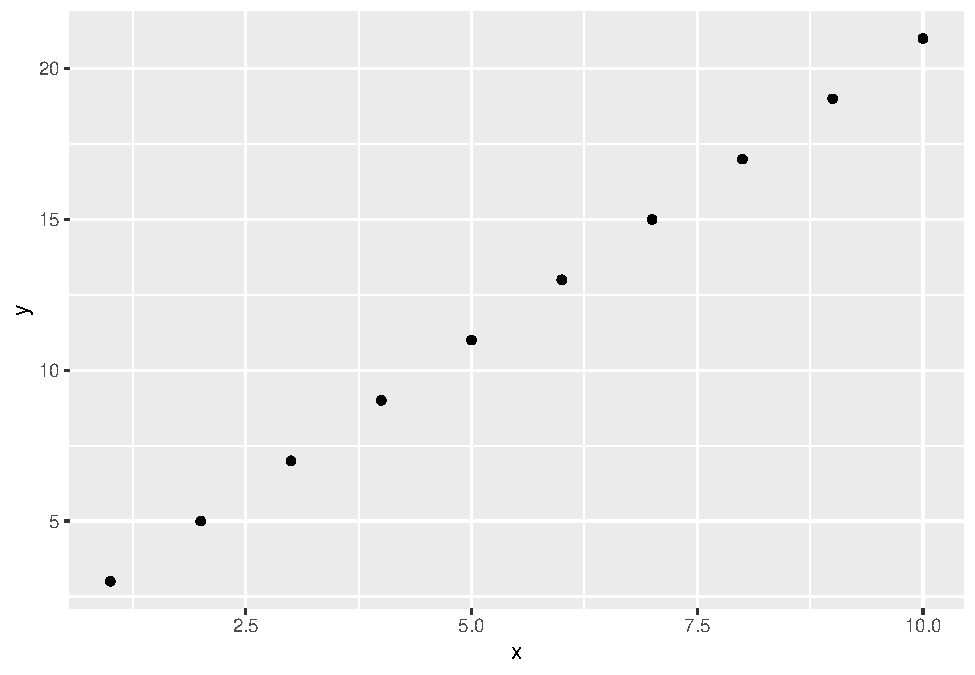
\includegraphics{main_files/figure-latex/unnamed-chunk-36-1.pdf}

Let us now plot a line to make our plot more informative and better looking.

\begin{Shaded}
\begin{Highlighting}[]
\CommentTok{\# Let us now plot x and y using ggplot2}
\FunctionTok{ggplot}\NormalTok{(}\AttributeTok{data=}\ConstantTok{NULL}\NormalTok{, }\FunctionTok{aes}\NormalTok{(x,y)) }\SpecialCharTok{+}
  \FunctionTok{geom\_point}\NormalTok{() }\SpecialCharTok{+}
  \FunctionTok{geom\_smooth}\NormalTok{(}\AttributeTok{method=}\StringTok{"lm"}\NormalTok{)}
\end{Highlighting}
\end{Shaded}

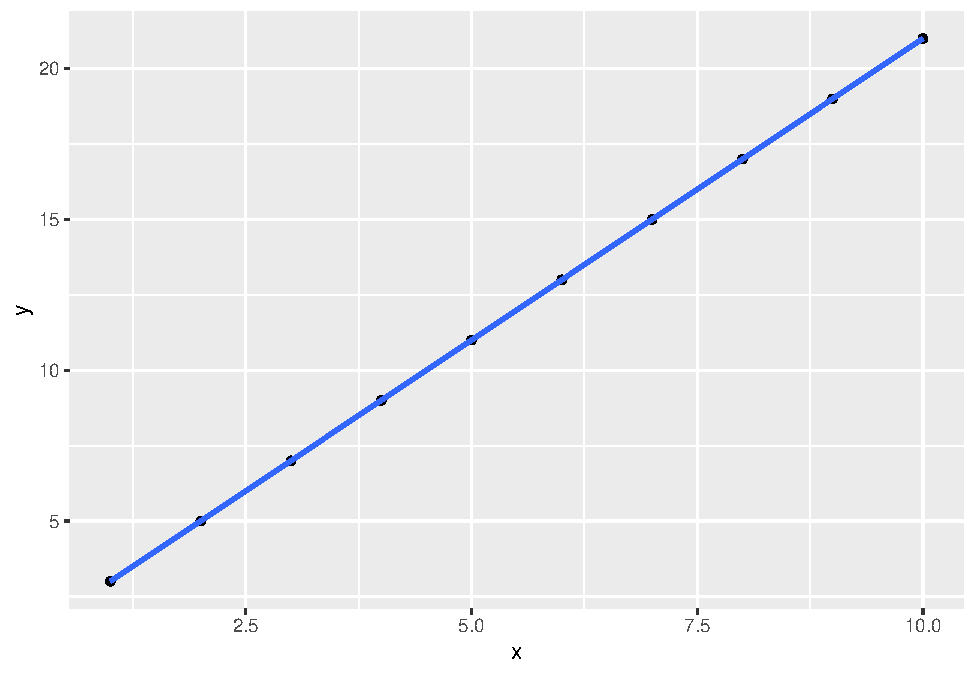
\includegraphics{main_files/figure-latex/unnamed-chunk-37-1.pdf}

Notice that playing with the scale sizes will yield dramatic changes in the effects we observe. For this, we can simply use the \texttt{xlim()} and \texttt{ylim()} functions to identify the lower and upper limits of x and y axes.

\begin{Shaded}
\begin{Highlighting}[]
\FunctionTok{ggplot}\NormalTok{(}\AttributeTok{data=}\ConstantTok{NULL}\NormalTok{, }\FunctionTok{aes}\NormalTok{(x,y)) }\SpecialCharTok{+}
  \FunctionTok{geom\_point}\NormalTok{() }\SpecialCharTok{+}
  \FunctionTok{geom\_smooth}\NormalTok{(}\AttributeTok{method=}\StringTok{"lm"}\NormalTok{)}\SpecialCharTok{+}
  \FunctionTok{xlim}\NormalTok{(}\DecValTok{0}\NormalTok{, }\DecValTok{15}\NormalTok{) }\SpecialCharTok{+}
  \FunctionTok{ylim}\NormalTok{(}\DecValTok{0}\NormalTok{,}\DecValTok{100}\NormalTok{)}
\end{Highlighting}
\end{Shaded}

\begin{verbatim}
## `geom_smooth()` using formula = 'y ~ x'
\end{verbatim}

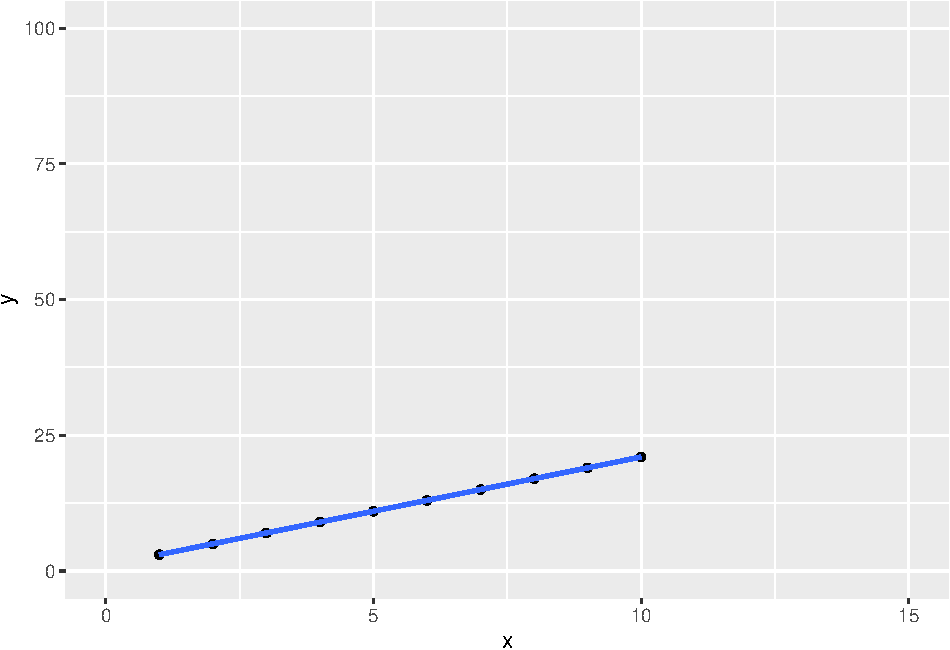
\includegraphics{main_files/figure-latex/unnamed-chunk-38-1.pdf}

Let us now plot a quadratic function. A quadratic function is one where the base is a variable and the exponent is constant. The following graph plots \texttt{n\^{}2}.

\begin{Shaded}
\begin{Highlighting}[]
\CommentTok{\# Let us now plot a and b using ggplot2}

\NormalTok{a}\OtherTok{\textless{}{-}} \DecValTok{1}\SpecialCharTok{:}\DecValTok{10}
\NormalTok{b }\OtherTok{\textless{}{-}}\NormalTok{ a}\SpecialCharTok{\^{}}\DecValTok{2}
\FunctionTok{ggplot}\NormalTok{(}\AttributeTok{data=}\ConstantTok{NULL}\NormalTok{, }\FunctionTok{aes}\NormalTok{(a,b)) }\SpecialCharTok{+}
  \FunctionTok{geom\_point}\NormalTok{() }\SpecialCharTok{+}
  \FunctionTok{geom\_smooth}\NormalTok{(}\AttributeTok{method=}\StringTok{"lm"}\NormalTok{,}\AttributeTok{formula =}\NormalTok{ y}\SpecialCharTok{\textasciitilde{}}\NormalTok{x }\SpecialCharTok{+}\FunctionTok{I}\NormalTok{(x}\SpecialCharTok{\^{}}\DecValTok{2}\NormalTok{), }\AttributeTok{color=}\StringTok{\textquotesingle{}orange\textquotesingle{}}\NormalTok{)}
\end{Highlighting}
\end{Shaded}

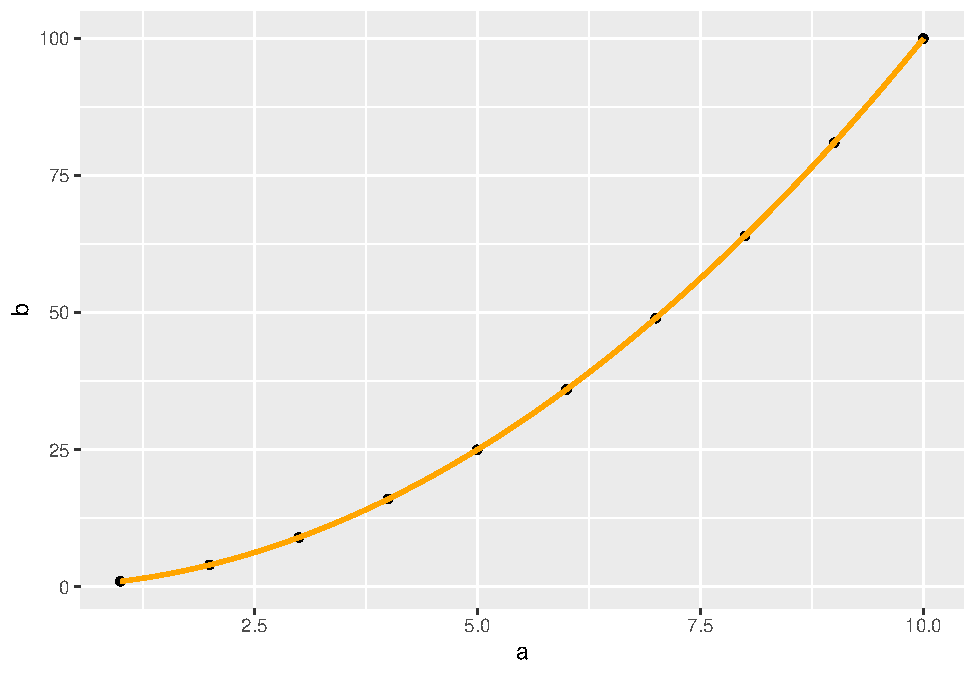
\includegraphics{main_files/figure-latex/unnamed-chunk-39-1.pdf}

Finally, we can plot an exponential function where the variable is the exponent and the base is constant.

\begin{Shaded}
\begin{Highlighting}[]
\CommentTok{\# Let us now plot a and b using ggplot2}

\NormalTok{a}\OtherTok{\textless{}{-}} \DecValTok{1}\SpecialCharTok{:}\DecValTok{10}
\NormalTok{b }\OtherTok{\textless{}{-}} \FunctionTok{exp}\NormalTok{(a)}
\FunctionTok{ggplot}\NormalTok{(}\AttributeTok{data=}\ConstantTok{NULL}\NormalTok{, }\FunctionTok{aes}\NormalTok{(a,b)) }\SpecialCharTok{+}
  \FunctionTok{geom\_point}\NormalTok{() }\SpecialCharTok{+}
  \FunctionTok{geom\_smooth}\NormalTok{(}\AttributeTok{method=}\StringTok{"lm"}\NormalTok{,}\AttributeTok{color =} \StringTok{"orange"}\NormalTok{,}\AttributeTok{formula=}\NormalTok{ (y }\SpecialCharTok{\textasciitilde{}} \FunctionTok{exp}\NormalTok{(x)))}
\end{Highlighting}
\end{Shaded}

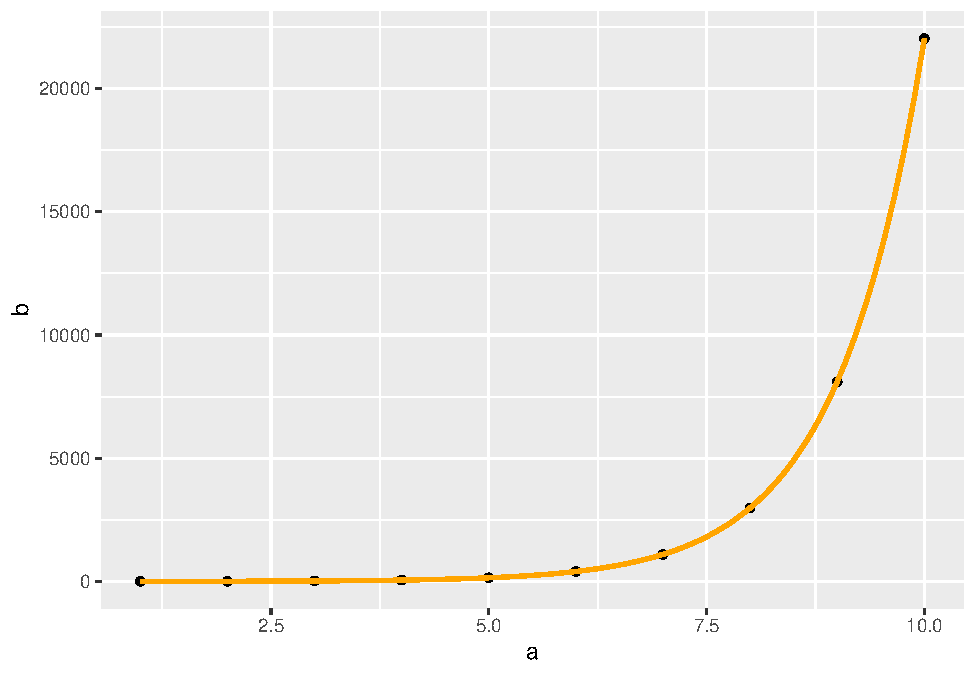
\includegraphics{main_files/figure-latex/unnamed-chunk-40-1.pdf}

You can mix and match.

\begin{Shaded}
\begin{Highlighting}[]
\CommentTok{\# Let us now plot x and y using ggplot2}
\NormalTok{a}\OtherTok{\textless{}{-}} \DecValTok{1}\SpecialCharTok{:}\DecValTok{10}
\NormalTok{b}\OtherTok{\textless{}{-}}\NormalTok{ a}\SpecialCharTok{\^{}}\DecValTok{2}
\FunctionTok{ggplot}\NormalTok{(}\AttributeTok{data=}\ConstantTok{NULL}\NormalTok{, }\FunctionTok{aes}\NormalTok{(x,y)) }\SpecialCharTok{+}
  \FunctionTok{geom\_smooth}\NormalTok{(}\AttributeTok{method=}\StringTok{"lm"}\NormalTok{) }\SpecialCharTok{+}
  \FunctionTok{geom\_smooth}\NormalTok{(}\AttributeTok{data=}\ConstantTok{NULL}\NormalTok{, }\FunctionTok{aes}\NormalTok{(a,b), }\AttributeTok{method=}\StringTok{"lm"}\NormalTok{, }\AttributeTok{formula =}\NormalTok{ y}\SpecialCharTok{\textasciitilde{}}\NormalTok{x }\SpecialCharTok{+}\FunctionTok{I}\NormalTok{(x}\SpecialCharTok{\^{}}\DecValTok{2}\NormalTok{),}\AttributeTok{color=} \StringTok{\textquotesingle{}orange\textquotesingle{}}\NormalTok{) }
\end{Highlighting}
\end{Shaded}

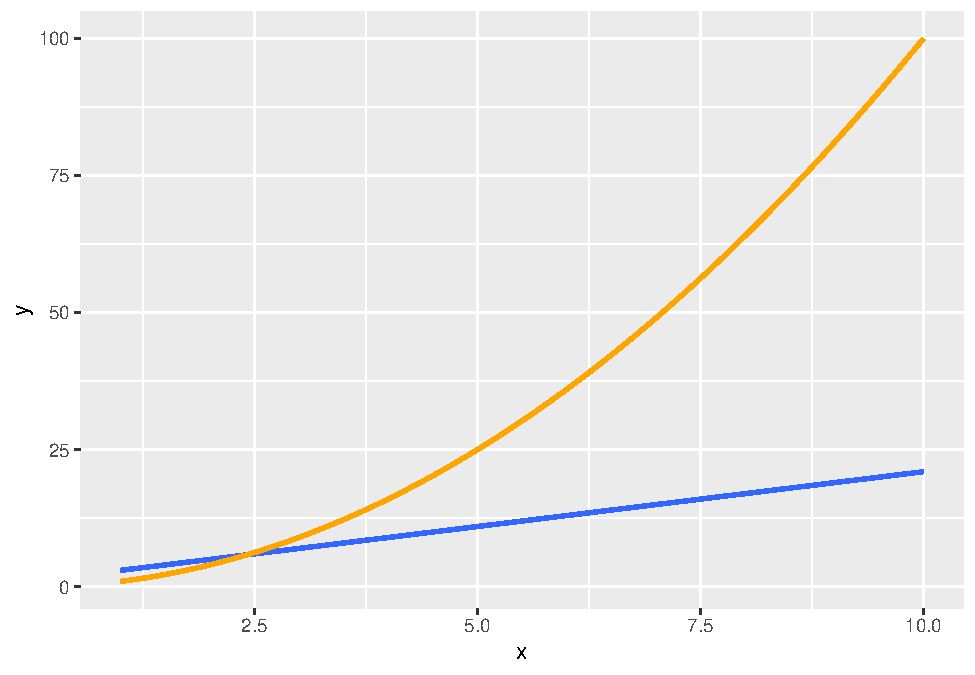
\includegraphics{main_files/figure-latex/unnamed-chunk-41-1.pdf}

\hypertarget{operators-and-functions-in-this-section}{%
\section{Operators and functions in this section}\label{operators-and-functions-in-this-section}}

\hypertarget{operators-1}{%
\subsection{Operators}\label{operators-1}}

\texttt{x\ +\ y}

Addition

\texttt{x\ -\ y}

Subtraction

\texttt{x\ *\ y}

Multiplication

\texttt{x\ /\ y}

Division

\texttt{x\^{}y}

Exponentiation

\texttt{x\ \textless{}-\ y}

Assignment

\texttt{==}

Test for equality. \textbf{Don't confuse with a single =, which is an assignment operator (and also always returns TRUE).}

\texttt{!=}

Test for inequality

\texttt{\textless{}}

Test, smaller than

\texttt{\textgreater{}}

Test, greater than

\texttt{\textless{}=}

Test, smaller than or equal to

\texttt{\textgreater{}=}

Test, greater than or equal to

\hypertarget{functions}{%
\subsection{Functions}\label{functions}}

\texttt{install.packages(package\_name)}

Installs one or several package(s).
The argument \texttt{package\_name} can either be a character (\texttt{install.packages(\textquotesingle{}dplyr\textquotesingle{})}) like or a character vector (\texttt{install.packages(c(\textquotesingle{}dplyr\textquotesingle{},\textquotesingle{}ggplot2\textquotesingle{}))}).

\texttt{library(package\_name)}

Loads a package called \texttt{package\_name}.

\hfill\break

\texttt{typeof(x)}

Determines the type of a variable/vector.

\hfill\break

\texttt{as.double(x)}

Converts a variable/vector to type \textbf{double}.

\hypertarget{data-structures}{%
\chapter{Data Structures}\label{data-structures}}

\hypertarget{data-types-in-r}{%
\section{Data Types in R}\label{data-types-in-r}}

In R, value has a \emph{type}:

\begin{longtable}[]{@{}
  >{\raggedleft\arraybackslash}p{(\columnwidth - 2\tabcolsep) * \real{0.2667}}
  >{\centering\arraybackslash}p{(\columnwidth - 2\tabcolsep) * \real{0.7333}}@{}}
\toprule\noalign{}
\begin{minipage}[b]{\linewidth}\raggedleft
Data Type
\end{minipage} & \begin{minipage}[b]{\linewidth}\centering
Examples
\end{minipage} \\
\midrule\noalign{}
\endhead
\bottomrule\noalign{}
\endlastfoot
Integer (Numeric): & \ldots, -3, -2, -1, 0, +1, +2, +3, \ldots{} \\
Double (Numeric): & most rational numbers; e.g., 1.0, 1.5, 20.0, pi \\
Character: & \texttt{"a"}, \texttt{"b"}, \texttt{"word"}, \texttt{"hello\ dear\ friend,\ ..."} \\
Logical: & \texttt{TRUE} or \texttt{FALSE} (or: \texttt{T} or \texttt{F} ) \\
Factor: & Restricted, user-defined set of values, internally represented numerically (e.g., Gender \{`male', `female', `other'\}) \\
Ordered factor: & Factor with an ordering (e.g., Starbucks coffee sizes \{`venti' \textgreater{} `grande' \textgreater{} `tall'\}) \\
\end{longtable}

\hypertarget{data-structures-in-r}{%
\section{Data Structures in R}\label{data-structures-in-r}}

\begin{itemize}
\item
  All values in R are organized in data structures. Structures differ in their number of dimensions and in whether they allow mixed data types.
\item
  In this course, we will mainly use vectors and data frames.
\end{itemize}

\begin{longtable}[]{@{}
  >{\raggedleft\arraybackslash}p{(\columnwidth - 6\tabcolsep) * \real{0.1667}}
  >{\centering\arraybackslash}p{(\columnwidth - 6\tabcolsep) * \real{0.3571}}
  >{\centering\arraybackslash}p{(\columnwidth - 6\tabcolsep) * \real{0.2381}}
  >{\centering\arraybackslash}p{(\columnwidth - 6\tabcolsep) * \real{0.2381}}@{}}
\toprule\noalign{}
\begin{minipage}[b]{\linewidth}\raggedleft
\end{minipage} & \begin{minipage}[b]{\linewidth}\centering
dimensions
\end{minipage} & \begin{minipage}[b]{\linewidth}\centering
types
\end{minipage} & \begin{minipage}[b]{\linewidth}\centering
\end{minipage} \\
\midrule\noalign{}
\endhead
\bottomrule\noalign{}
\endlastfoot
Vector & 1-dimensional & one type & 
\includegraphics[width=0.25\textwidth,height=\textheight]{img/vector.jpg} \\
Matrix & 2-dimensional & one type & 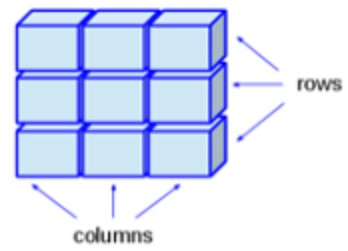
\includegraphics[width=0.2\textwidth,height=\textheight]{img/matrix.jpg} \\
Array & n-dimensional & one type & 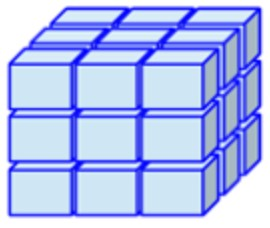
\includegraphics[width=0.2\textwidth,height=\textheight]{img/array.jpg} \\
Data frame (or tibble) & 2-dimensional & mixed types & 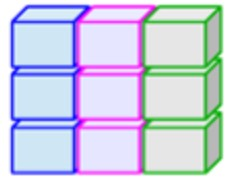
\includegraphics[width=0.2\textwidth,height=\textheight]{img/data_frame.jpg} \\
List & 1-dimensional & mixed types & 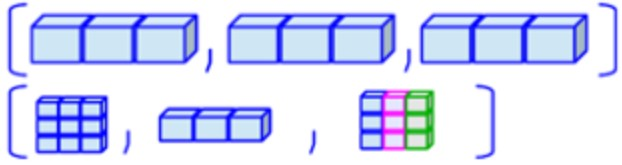
\includegraphics[width=0.5\textwidth,height=\textheight]{img/list.jpg} \\
\end{longtable}

(Illustrations from Gaurav Tiwari's article on medium \href{https://medium.com/@tiwarigaurav2512/r-data-types-847fffb01d5b}{here}.)

\begin{itemize}
\tightlist
\item
  Let's look at some examples
\end{itemize}

\begin{Shaded}
\begin{Highlighting}[]
\CommentTok{\# create and print vectors, don\textquotesingle{}t save}
\FunctionTok{c}\NormalTok{(}\DecValTok{1}\NormalTok{,}\DecValTok{2}\NormalTok{, }\DecValTok{1000}\NormalTok{)}
\end{Highlighting}
\end{Shaded}

\begin{Shaded}
\begin{Highlighting}[]
\NormalTok{\#\# [1]    1    2 1000}
\end{Highlighting}
\end{Shaded}

\begin{Shaded}
\begin{Highlighting}[]
\FunctionTok{c}\NormalTok{(}\DecValTok{1}\NormalTok{,}\DecValTok{2}\NormalTok{, }\DecValTok{1000}\NormalTok{, pi)}
\end{Highlighting}
\end{Shaded}

\begin{Shaded}
\begin{Highlighting}[]
\NormalTok{\#\# [1]    1.000000    2.000000 1000.000000    3.141593}
\end{Highlighting}
\end{Shaded}

\begin{Shaded}
\begin{Highlighting}[]
\DecValTok{1}\SpecialCharTok{:}\DecValTok{3}
\end{Highlighting}
\end{Shaded}

\begin{Shaded}
\begin{Highlighting}[]
\NormalTok{\#\# [1] 1 2 3}
\end{Highlighting}
\end{Shaded}

\begin{Shaded}
\begin{Highlighting}[]
\CommentTok{\# create and print a data.frame}
\FunctionTok{data.frame}\NormalTok{(}\DecValTok{1}\SpecialCharTok{:}\DecValTok{3}\NormalTok{)}
\end{Highlighting}
\end{Shaded}

\begin{Shaded}
\begin{Highlighting}[]
\NormalTok{\#\#   X1.3}
\NormalTok{\#\# 1    1}
\NormalTok{\#\# 2    2}
\NormalTok{\#\# 3    3}
\end{Highlighting}
\end{Shaded}

\hypertarget{vectors}{%
\section{Vectors}\label{vectors}}

\begin{itemize}
\tightlist
\item
  Vectors are simply ordered lists of elements, where every element has the same type.
\item
  They are useful for storing sets or sequences of numbers.
\item
  Let's create a simple vector with all integers from 1 to 8 and look at its contents.
\end{itemize}

\begin{Shaded}
\begin{Highlighting}[]
\NormalTok{vector\_var }\OtherTok{\textless{}{-}} \FunctionTok{c}\NormalTok{(}\DecValTok{1}\NormalTok{,}\DecValTok{2}\NormalTok{,}\DecValTok{3}\NormalTok{,}\DecValTok{4}\NormalTok{,}\DecValTok{5}\NormalTok{,}\DecValTok{6}\NormalTok{,}\DecValTok{7}\NormalTok{,}\DecValTok{8}\NormalTok{)}
\NormalTok{vector\_var}
\end{Highlighting}
\end{Shaded}

\begin{Shaded}
\begin{Highlighting}[]
\NormalTok{\#\# [1] 1 2 3 4 5 6 7 8}
\end{Highlighting}
\end{Shaded}

\begin{itemize}
\tightlist
\item
  There is even a more elegant ways to do that:
\end{itemize}

\begin{Shaded}
\begin{Highlighting}[]
\NormalTok{vector\_var }\OtherTok{\textless{}{-}} \DecValTok{1}\SpecialCharTok{:}\DecValTok{8}
\NormalTok{vector\_var}
\end{Highlighting}
\end{Shaded}

\begin{Shaded}
\begin{Highlighting}[]
\NormalTok{\#\# [1] 1 2 3 4 5 6 7 8}
\end{Highlighting}
\end{Shaded}

\begin{itemize}
\tightlist
\item
  Now, let's create a simple vector with integers between 1 and 8, going in steps of 2.
\end{itemize}

\begin{Shaded}
\begin{Highlighting}[]
\NormalTok{vector\_var }\OtherTok{\textless{}{-}} \FunctionTok{seq}\NormalTok{(}\DecValTok{1}\NormalTok{,}\DecValTok{8}\NormalTok{, }\AttributeTok{by=}\DecValTok{2}\NormalTok{)}
\NormalTok{vector\_var}
\end{Highlighting}
\end{Shaded}

\begin{Shaded}
\begin{Highlighting}[]
\NormalTok{\#\# [1] 1 3 5 7}
\end{Highlighting}
\end{Shaded}

\begin{itemize}
\tightlist
\item
  Some useful vectors already exist in R.
\end{itemize}

\begin{Shaded}
\begin{Highlighting}[]
\NormalTok{letters}
\end{Highlighting}
\end{Shaded}

\begin{Shaded}
\begin{Highlighting}[]
\NormalTok{\#\#  [1] "a" "b" "c" "d" "e" "f" "g" "h" "i" "j" "k" "l" "m" "n" "o" "p" "q" "r" "s"}
\NormalTok{\#\# [20] "t" "u" "v" "w" "x" "y" "z"}
\end{Highlighting}
\end{Shaded}

\begin{Shaded}
\begin{Highlighting}[]
\NormalTok{LETTERS}
\end{Highlighting}
\end{Shaded}

\begin{Shaded}
\begin{Highlighting}[]
\NormalTok{\#\#  [1] "A" "B" "C" "D" "E" "F" "G" "H" "I" "J" "K" "L" "M" "N" "O" "P" "Q" "R" "S"}
\NormalTok{\#\# [20] "T" "U" "V" "W" "X" "Y" "Z"}
\end{Highlighting}
\end{Shaded}

\begin{itemize}
\tightlist
\item
  We can select specific elements of a vector by indexing it with \texttt{{[}{]}}.
\end{itemize}

\begin{Shaded}
\begin{Highlighting}[]
\CommentTok{\# the first letter}
\NormalTok{letters[}\DecValTok{1}\NormalTok{]}
\end{Highlighting}
\end{Shaded}

\begin{Shaded}
\begin{Highlighting}[]
\NormalTok{\#\# [1] "a"}
\end{Highlighting}
\end{Shaded}

\begin{Shaded}
\begin{Highlighting}[]
\CommentTok{\# the 13{-}th letter}
\NormalTok{letters[}\DecValTok{13}\NormalTok{]}
\end{Highlighting}
\end{Shaded}

\begin{Shaded}
\begin{Highlighting}[]
\NormalTok{\#\# [1] "m"}
\end{Highlighting}
\end{Shaded}

\begin{itemize}
\tightlist
\item
  Indices can be vectors too.
\end{itemize}

\begin{Shaded}
\begin{Highlighting}[]
\CommentTok{\# both of them}
\NormalTok{letters[}\FunctionTok{c}\NormalTok{(}\DecValTok{1}\NormalTok{,}\DecValTok{7}\NormalTok{)]}
\end{Highlighting}
\end{Shaded}

\begin{Shaded}
\begin{Highlighting}[]
\NormalTok{\#\# [1] "a" "g"}
\end{Highlighting}
\end{Shaded}

\begin{itemize}
\tightlist
\item
  We can even take a whole \emph{`slice'} of a vector.
\end{itemize}

\begin{Shaded}
\begin{Highlighting}[]
\CommentTok{\# both of them}
\NormalTok{letters[}\DecValTok{6}\SpecialCharTok{:}\DecValTok{12}\NormalTok{]}
\end{Highlighting}
\end{Shaded}

\begin{Shaded}
\begin{Highlighting}[]
\NormalTok{\#\# [1] "f" "g" "h" "i" "j" "k" "l"}
\end{Highlighting}
\end{Shaded}

\begin{itemize}
\tightlist
\item
  Indices can even be negative. A negative index \(-n\) means \emph{`everything' except \(n\)}.
\end{itemize}

\begin{Shaded}
\begin{Highlighting}[]
\CommentTok{\# both of them}
\NormalTok{letters[}\SpecialCharTok{{-}}\DecValTok{1}\NormalTok{]}
\end{Highlighting}
\end{Shaded}

\begin{Shaded}
\begin{Highlighting}[]
\NormalTok{\#\#  [1] "b" "c" "d" "e" "f" "g" "h" "i" "j" "k" "l" "m" "n" "o" "p" "q" "r" "s" "t"}
\NormalTok{\#\# [20] "u" "v" "w" "x" "y" "z"}
\end{Highlighting}
\end{Shaded}

\begin{itemize}
\tightlist
\item
  Vectors can be named.
\end{itemize}

\begin{Shaded}
\begin{Highlighting}[]
\NormalTok{digits }\OtherTok{\textless{}{-}} \FunctionTok{c}\NormalTok{(}\StringTok{\textquotesingle{}one\textquotesingle{}}\OtherTok{=}\DecValTok{1}\NormalTok{, }\StringTok{\textquotesingle{}two\textquotesingle{}}\OtherTok{=}\DecValTok{2}\NormalTok{, }\StringTok{\textquotesingle{}three\textquotesingle{}}\OtherTok{=}\DecValTok{3}\NormalTok{, }\StringTok{\textquotesingle{}four\textquotesingle{}}\OtherTok{=}\DecValTok{4}\NormalTok{, }\StringTok{\textquotesingle{}five\textquotesingle{}}\OtherTok{=}\DecValTok{5}\NormalTok{, }\StringTok{\textquotesingle{}six\textquotesingle{}}\OtherTok{=}\DecValTok{6}\NormalTok{)}
\end{Highlighting}
\end{Shaded}

\begin{itemize}
\tightlist
\item
  In this case, we can index by the name
\end{itemize}

\begin{Shaded}
\begin{Highlighting}[]
\NormalTok{digits[}\FunctionTok{c}\NormalTok{(}\StringTok{\textquotesingle{}one\textquotesingle{}}\NormalTok{, }\StringTok{\textquotesingle{}six\textquotesingle{}}\NormalTok{)]}
\end{Highlighting}
\end{Shaded}

\begin{Shaded}
\begin{Highlighting}[]
\NormalTok{\#\# one six }
\NormalTok{\#\#   1   6}
\end{Highlighting}
\end{Shaded}

\begin{itemize}
\tightlist
\item
  Believe it or not, everything in R is actually a vector. For example \texttt{9} is a vector with only one element, which is \texttt{9}.
\end{itemize}

\begin{Shaded}
\begin{Highlighting}[]
\DecValTok{9}
\end{Highlighting}
\end{Shaded}

\begin{Shaded}
\begin{Highlighting}[]
\NormalTok{\#\# [1] 9}
\end{Highlighting}
\end{Shaded}

\begin{itemize}
\tightlist
\item
  This is why every output begins with \texttt{{[}1{]}}. R tries to help you find numbers in printed vectors. Every time a vector is printed, it reminds you at which position in the vector we are.
\item
  The \texttt{{[}1{]}} in the output below tells you that \texttt{"a"} is the first element, and the \texttt{{[}20{]}} tells you that \texttt{"t"} is the 20-th element.
\end{itemize}

\begin{Shaded}
\begin{Highlighting}[]
\NormalTok{letters }\CommentTok{\# print a vector with all lower{-}case letters}
\end{Highlighting}
\end{Shaded}

\begin{Shaded}
\begin{Highlighting}[]
\NormalTok{\#\#  [1] "a" "b" "c" "d" "e" "f" "g" "h" "i" "j" "k" "l" "m" "n" "o" "p" "q" "r" "s"}
\NormalTok{\#\# [20] "t" "u" "v" "w" "x" "y" "z"}
\end{Highlighting}
\end{Shaded}

\hypertarget{what-are-vectors-good-for}{%
\subsection{What are vectors good for?}\label{what-are-vectors-good-for}}

\begin{itemize}
\tightlist
\item
  Let's put this knowledge to use.
\item
  Here are two vectors representing the winnings from my recent gambling:
\end{itemize}

\begin{Shaded}
\begin{Highlighting}[]
\NormalTok{horse\_bets\_payout\_tl }\OtherTok{\textless{}{-}} \FunctionTok{c}\NormalTok{(}\DecValTok{100}\NormalTok{, }\SpecialCharTok{{-}}\DecValTok{50}\NormalTok{, }\DecValTok{1}\NormalTok{, }\DecValTok{100}\NormalTok{, }\SpecialCharTok{{-}}\DecValTok{10}\NormalTok{, }\SpecialCharTok{{-}}\DecValTok{20}\NormalTok{, }\DecValTok{250}\NormalTok{, }\SpecialCharTok{{-}}\DecValTok{40}\NormalTok{, }\SpecialCharTok{{-}}\DecValTok{30}\NormalTok{, }\DecValTok{23}\NormalTok{, }\SpecialCharTok{{-}}\DecValTok{23}\NormalTok{, }\DecValTok{55}\NormalTok{, }\DecValTok{14}\NormalTok{, }\DecValTok{8}\NormalTok{, }\DecValTok{24}\NormalTok{, }\SpecialCharTok{{-}}\DecValTok{3}\NormalTok{)}
\end{Highlighting}
\end{Shaded}

\begin{Shaded}
\begin{Highlighting}[]
\NormalTok{poker\_payout\_tl }\OtherTok{\textless{}{-}} \FunctionTok{c}\NormalTok{(}\DecValTok{24}\NormalTok{, }\DecValTok{5}\NormalTok{, }\SpecialCharTok{{-}}\FloatTok{38.1}\NormalTok{, }\DecValTok{12}\NormalTok{, }\DecValTok{103}\NormalTok{, }\DecValTok{15}\NormalTok{, }\DecValTok{5}\NormalTok{, }\DecValTok{187}\NormalTok{, }\DecValTok{13}\NormalTok{, }\SpecialCharTok{{-}}\DecValTok{23}\NormalTok{, }\SpecialCharTok{{-}}\DecValTok{45}\NormalTok{, }\DecValTok{36}\NormalTok{)}
\end{Highlighting}
\end{Shaded}

\begin{itemize}
\tightlist
\item
  Let's find out which game is more profitable.
\item
  To get our average profit, we first need to compute the sum of a vector.
\item
  Then, we will divide the sum by the length of the vector.
\item
  First, let's compute the sums of these vectors.
\end{itemize}

\begin{Shaded}
\begin{Highlighting}[]
\FunctionTok{sum}\NormalTok{(horse\_bets\_payout\_tl)}
\end{Highlighting}
\end{Shaded}

\begin{Shaded}
\begin{Highlighting}[]
\NormalTok{\#\# [1] 399}
\end{Highlighting}
\end{Shaded}

\begin{Shaded}
\begin{Highlighting}[]
\FunctionTok{sum}\NormalTok{(poker\_payout\_tl)}
\end{Highlighting}
\end{Shaded}

\begin{Shaded}
\begin{Highlighting}[]
\NormalTok{\#\# [1] 293.9}
\end{Highlighting}
\end{Shaded}

\begin{itemize}
\tightlist
\item
  Now, we need to determine the length of these vectors:
\end{itemize}

\begin{Shaded}
\begin{Highlighting}[]
\FunctionTok{length}\NormalTok{(horse\_bets\_payout\_tl)}
\end{Highlighting}
\end{Shaded}

\begin{Shaded}
\begin{Highlighting}[]
\NormalTok{\#\# [1] 16}
\end{Highlighting}
\end{Shaded}

\begin{Shaded}
\begin{Highlighting}[]
\FunctionTok{length}\NormalTok{(poker\_payout\_tl)}
\end{Highlighting}
\end{Shaded}

\begin{Shaded}
\begin{Highlighting}[]
\NormalTok{\#\# [1] 12}
\end{Highlighting}
\end{Shaded}

\begin{itemize}
\tightlist
\item
  Dividing the sum by the length would give us our average profit.
\end{itemize}

\begin{Shaded}
\begin{Highlighting}[]
\FunctionTok{sum}\NormalTok{(horse\_bets\_payout\_tl)}\SpecialCharTok{/}\FunctionTok{length}\NormalTok{(horse\_bets\_payout\_tl)}
\end{Highlighting}
\end{Shaded}

\begin{Shaded}
\begin{Highlighting}[]
\NormalTok{\#\# [1] 24.9375}
\end{Highlighting}
\end{Shaded}

\begin{Shaded}
\begin{Highlighting}[]
\FunctionTok{sum}\NormalTok{(poker\_payout\_tl)}\SpecialCharTok{/}\FunctionTok{length}\NormalTok{(poker\_payout\_tl)}
\end{Highlighting}
\end{Shaded}

\begin{Shaded}
\begin{Highlighting}[]
\NormalTok{\#\# [1] 24.49167}
\end{Highlighting}
\end{Shaded}

\ldots{} so which game is more profitable?

\begin{itemize}
\item
  It seems that betting is more profitable.
\item
  Next time, we can accomplish this calulation by calling the function \texttt{mean()}.
\end{itemize}

\begin{Shaded}
\begin{Highlighting}[]
\FunctionTok{mean}\NormalTok{(horse\_bets\_payout\_tl)}
\end{Highlighting}
\end{Shaded}

\begin{Shaded}
\begin{Highlighting}[]
\NormalTok{\#\# [1] 24.9375}
\end{Highlighting}
\end{Shaded}

\begin{Shaded}
\begin{Highlighting}[]
\FunctionTok{mean}\NormalTok{(poker\_payout\_tl)}
\end{Highlighting}
\end{Shaded}

\begin{Shaded}
\begin{Highlighting}[]
\NormalTok{\#\# [1] 24.49167}
\end{Highlighting}
\end{Shaded}

\ldots Now, I forgot to mention that my bookie charges me 1.5 TL per bet on a horse, on average. The poker payouts correspond to the profits, though. \ldots 

\begin{itemize}
\item
  Luckily, we can just add numbers and vectors. Let's just create two new vectors which contain the profits.
\item
  Let's subtract 1.5 from elements of \texttt{horse\_bets\_payout\_tl} and save the result as \texttt{horse\_bets\_profits\_tl}.
\item
  As you see, this subtraction is applied to every element of the vector.
\end{itemize}

\begin{Shaded}
\begin{Highlighting}[]
\NormalTok{horse\_bets\_profits\_tl }\OtherTok{\textless{}{-}}\NormalTok{ horse\_bets\_payout\_tl }\SpecialCharTok{{-}} \FloatTok{1.5}
\FunctionTok{head}\NormalTok{(horse\_bets\_profits\_tl)}
\end{Highlighting}
\end{Shaded}

\begin{Shaded}
\begin{Highlighting}[]
\NormalTok{\#\# [1]  98.5 {-}51.5  {-}0.5  98.5 {-}11.5 {-}21.5}
\end{Highlighting}
\end{Shaded}

\begin{Shaded}
\begin{Highlighting}[]
\FunctionTok{head}\NormalTok{(horse\_bets\_payout\_tl)}
\end{Highlighting}
\end{Shaded}

\begin{Shaded}
\begin{Highlighting}[]
\NormalTok{\#\# [1] 100 {-}50   1 100 {-}10 {-}20}
\end{Highlighting}
\end{Shaded}

\begin{itemize}
\tightlist
\item
  For poker, we don't need to change anything. So, we assign the already existing \texttt{poker\_payout\_tl} vector to another vector called \texttt{poker\_profits\_tl}.
\end{itemize}

\begin{Shaded}
\begin{Highlighting}[]
\NormalTok{poker\_profits\_tl }\OtherTok{\textless{}{-}}\NormalTok{ poker\_payout\_tl}
\end{Highlighting}
\end{Shaded}

\begin{itemize}
\tightlist
\item
  Let's compare:
\end{itemize}

\begin{Shaded}
\begin{Highlighting}[]
\NormalTok{horse\_bets\_payout\_tl}
\end{Highlighting}
\end{Shaded}

\begin{Shaded}
\begin{Highlighting}[]
\NormalTok{\#\#  [1] 100 {-}50   1 100 {-}10 {-}20 250 {-}40 {-}30  23 {-}23  55  14   8  24  {-}3}
\end{Highlighting}
\end{Shaded}

\begin{Shaded}
\begin{Highlighting}[]
\NormalTok{horse\_bets\_profits\_tl}
\end{Highlighting}
\end{Shaded}

\begin{Shaded}
\begin{Highlighting}[]
\NormalTok{\#\#  [1]  98.5 {-}51.5  {-}0.5  98.5 {-}11.5 {-}21.5 248.5 {-}41.5 {-}31.5  21.5 {-}24.5  53.5}
\NormalTok{\#\# [13]  12.5   6.5  22.5  {-}4.5}
\end{Highlighting}
\end{Shaded}

\begin{Shaded}
\begin{Highlighting}[]
\NormalTok{poker\_payout\_tl}
\end{Highlighting}
\end{Shaded}

\begin{Shaded}
\begin{Highlighting}[]
\NormalTok{\#\#  [1]  24.0   5.0 {-}38.1  12.0 103.0  15.0   5.0 187.0  13.0 {-}23.0 {-}45.0  36.0}
\end{Highlighting}
\end{Shaded}

\begin{Shaded}
\begin{Highlighting}[]
\NormalTok{poker\_profits\_tl}
\end{Highlighting}
\end{Shaded}

\begin{Shaded}
\begin{Highlighting}[]
\NormalTok{\#\#  [1]  24.0   5.0 {-}38.1  12.0 103.0  15.0   5.0 187.0  13.0 {-}23.0 {-}45.0  36.0}
\end{Highlighting}
\end{Shaded}

\begin{itemize}
\tightlist
\item
  Which game is more profitable now?
\end{itemize}

\begin{Shaded}
\begin{Highlighting}[]
\FunctionTok{mean}\NormalTok{(horse\_bets\_profits\_tl)}
\end{Highlighting}
\end{Shaded}

\begin{Shaded}
\begin{Highlighting}[]
\NormalTok{\#\# [1] 23.4375}
\end{Highlighting}
\end{Shaded}

\begin{Shaded}
\begin{Highlighting}[]
\FunctionTok{mean}\NormalTok{(poker\_profits\_tl)}
\end{Highlighting}
\end{Shaded}

\begin{Shaded}
\begin{Highlighting}[]
\NormalTok{\#\# [1] 24.49167}
\end{Highlighting}
\end{Shaded}

\hypertarget{data-frames}{%
\section{Data Frames}\label{data-frames}}

\begin{itemize}
\tightlist
\item
  What I forgot to mention is that I generally gamble on Wednesdays and Fridays. Maybe that matters?
\item
  How can we associate this information with the profits vectors?
\end{itemize}

\begin{itemize}
\tightlist
\item
  One way is to represent it in two vectors containing days of the week. In that case, every \(i\)-th element in \texttt{poker\_week\_days} corresponds to the \(i\)-th element in \texttt{poker\_week\_days}.
\end{itemize}

\begin{Shaded}
\begin{Highlighting}[]
\CommentTok{\# create two vectors with week days}
\NormalTok{horse\_bets\_week\_days }\OtherTok{\textless{}{-}} \FunctionTok{rep}\NormalTok{(}\FunctionTok{c}\NormalTok{(}\StringTok{"Wed"}\NormalTok{, }\StringTok{"Fr"}\NormalTok{), }\DecValTok{8}\NormalTok{)}
\NormalTok{poker\_week\_days }\OtherTok{\textless{}{-}} \FunctionTok{rep}\NormalTok{(}\FunctionTok{c}\NormalTok{(}\StringTok{"Wed"}\NormalTok{, }\StringTok{"Fr"}\NormalTok{), }\DecValTok{6}\NormalTok{)}
\end{Highlighting}
\end{Shaded}

\begin{itemize}
\item
  But this is getting messy. We have to keep track of two pairs a vectors, and the relations between them. Let's represent all poker-related information in one data structure, and all horse race-related information in another structure.
\item
  The best way to represent a pair of vectors where the \(i\)-th element in vector 1 corresponds to the \(i\)-th element in vector 2 is with data frames. We can create a new data frame with the function \texttt{data.frame()}.
\end{itemize}

\begin{Shaded}
\begin{Highlighting}[]
\NormalTok{df\_horse\_bets }\OtherTok{\textless{}{-}} 
  \FunctionTok{data.frame}\NormalTok{(}\AttributeTok{wday =}\NormalTok{ horse\_bets\_week\_days, }
             \AttributeTok{profit =}\NormalTok{ horse\_bets\_profits\_tl)}
\end{Highlighting}
\end{Shaded}

\begin{Shaded}
\begin{Highlighting}[]
\NormalTok{df\_poker }\OtherTok{\textless{}{-}} 
  \FunctionTok{data.frame}\NormalTok{(}\AttributeTok{wday =}\NormalTok{ poker\_week\_days, }
             \AttributeTok{profit =}\NormalTok{ poker\_payout\_tl)}
\end{Highlighting}
\end{Shaded}

\begin{itemize}
\tightlist
\item
  Let's take a look at what we've created.
\end{itemize}

\begin{Shaded}
\begin{Highlighting}[]
\NormalTok{df\_horse\_bets}
\end{Highlighting}
\end{Shaded}

\begin{Shaded}
\begin{Highlighting}[]
\NormalTok{\#\#    wday profit}
\NormalTok{\#\# 1   Wed   98.5}
\NormalTok{\#\# 2    Fr  {-}51.5}
\NormalTok{\#\# 3   Wed   {-}0.5}
\NormalTok{\#\# 4    Fr   98.5}
\NormalTok{\#\# 5   Wed  {-}11.5}
\NormalTok{\#\# 6    Fr  {-}21.5}
\NormalTok{\#\# 7   Wed  248.5}
\NormalTok{\#\# 8    Fr  {-}41.5}
\NormalTok{\#\# 9   Wed  {-}31.5}
\NormalTok{\#\# 10   Fr   21.5}
\NormalTok{\#\# 11  Wed  {-}24.5}
\NormalTok{\#\# 12   Fr   53.5}
\NormalTok{\#\# 13  Wed   12.5}
\NormalTok{\#\# 14   Fr    6.5}
\NormalTok{\#\# 15  Wed   22.5}
\NormalTok{\#\# 16   Fr   {-}4.5}
\end{Highlighting}
\end{Shaded}

\begin{itemize}
\item
  Wow. That's a rather long output \ldots{}
\item
  Generally, it's sufficient to see the first couple of rows of a \texttt{data.frame} to get a sense of what it contains.
\item
  We'll use the function \texttt{head()}, which takes a \texttt{data.frame} and a number \(n\), and outputs the first \(n\) lines.
\end{itemize}

\begin{Shaded}
\begin{Highlighting}[]
\CommentTok{\# let\textquotesingle{}s see the first two rows of the data frame called df\_horse\_bets}
\FunctionTok{head}\NormalTok{(df\_horse\_bets, }\DecValTok{2}\NormalTok{) }
\end{Highlighting}
\end{Shaded}

\begin{Shaded}
\begin{Highlighting}[]
\NormalTok{\#\#   wday profit}
\NormalTok{\#\# 1  Wed   98.5}
\NormalTok{\#\# 2   Fr  {-}51.5}
\end{Highlighting}
\end{Shaded}

\begin{itemize}
\tightlist
\item
  An alternative is \texttt{View()}, which shows you the entire \texttt{data.frame} within a new tab in the RStudio GUI.
\end{itemize}

\begin{Shaded}
\begin{Highlighting}[]
\FunctionTok{View}\NormalTok{(df\_poker)}
\end{Highlighting}
\end{Shaded}

\begin{itemize}
\item
  Turning back to our gambling example, we still have two objects, which really belong together.
\item
  Let's merge them into one long data frame.
\item
  The function \texttt{rbind()} takes two data frames as its arguments, and returns a single concatenated data frame, where all the rows of the first data frame are on top, and all the rows of the second data frame are at the bottom.
\end{itemize}

\begin{Shaded}
\begin{Highlighting}[]
\NormalTok{df\_gambling }\OtherTok{\textless{}{-}} \FunctionTok{rbind}\NormalTok{(df\_horse\_bets, df\_poker)}
\end{Highlighting}
\end{Shaded}

\begin{itemize}
\tightlist
\item
  Unfortunately, now, we don't have any information on which profits are from which game.
\end{itemize}

\begin{Shaded}
\begin{Highlighting}[]
\FunctionTok{head}\NormalTok{(df\_gambling)}
\end{Highlighting}
\end{Shaded}

\begin{Shaded}
\begin{Highlighting}[]
\NormalTok{\#\#   wday profit}
\NormalTok{\#\# 1  Wed   98.5}
\NormalTok{\#\# 2   Fr  {-}51.5}
\NormalTok{\#\# 3  Wed   {-}0.5}
\NormalTok{\#\# 4   Fr   98.5}
\NormalTok{\#\# 5  Wed  {-}11.5}
\NormalTok{\#\# 6   Fr  {-}21.5}
\end{Highlighting}
\end{Shaded}

\begin{itemize}
\tightlist
\item
  Let's fix this problem by enriching both data frames with this information.
\item
  We can assign to new (or old) columns with our assignment operator \texttt{\textless{}-}.
\item
  When we assign a value to a specific column, R puts the specified value into every row of the column of the given data frame.
\item
  What the following code says is ``Create a new column named \texttt{game} in the data frame named \texttt{df\_horse\_bets} and fill the column with the string \emph{horse\_bets}.''
\end{itemize}

\begin{Shaded}
\begin{Highlighting}[]
\NormalTok{df\_horse\_bets}\SpecialCharTok{$}\NormalTok{game }\OtherTok{\textless{}{-}} \StringTok{"horse\_bets"}
\NormalTok{df\_poker}\SpecialCharTok{$}\NormalTok{game }\OtherTok{\textless{}{-}} \StringTok{"poker"}
\end{Highlighting}
\end{Shaded}

\begin{itemize}
\tightlist
\item
  Now, let's bind them together again. (This overwrites the old data frame called \texttt{df\_gambling}, which we created previously.)
\end{itemize}

\begin{Shaded}
\begin{Highlighting}[]
\NormalTok{df\_gambling }\OtherTok{\textless{}{-}} \FunctionTok{rbind}\NormalTok{(df\_horse\_bets, df\_poker)}
\FunctionTok{head}\NormalTok{(df\_gambling)}
\end{Highlighting}
\end{Shaded}

\begin{Shaded}
\begin{Highlighting}[]
\NormalTok{\#\#   wday profit       game}
\NormalTok{\#\# 1  Wed   98.5 horse\_bets}
\NormalTok{\#\# 2   Fr  {-}51.5 horse\_bets}
\NormalTok{\#\# 3  Wed   {-}0.5 horse\_bets}
\NormalTok{\#\# 4   Fr   98.5 horse\_bets}
\NormalTok{\#\# 5  Wed  {-}11.5 horse\_bets}
\NormalTok{\#\# 6   Fr  {-}21.5 horse\_bets}
\end{Highlighting}
\end{Shaded}

\hypertarget{working-with-data-frames}{%
\section{Working with data frames}\label{working-with-data-frames}}

\begin{itemize}
\tightlist
\item
  Now, we can do very cool things very easily.
\item
  But we'll need two packages for that: \texttt{dplyr}, and \texttt{magrittr}.
\end{itemize}

\begin{Shaded}
\begin{Highlighting}[]
\CommentTok{\# load the two packages}
\FunctionTok{library}\NormalTok{(magrittr) }\CommentTok{\# for \textquotesingle{}\%\textgreater{}\%\textquotesingle{}}
\end{Highlighting}
\end{Shaded}

\begin{verbatim}
## 
## Attaching package: 'magrittr'
\end{verbatim}

\begin{verbatim}
## The following object is masked from 'package:purrr':
## 
##     set_names
\end{verbatim}

\begin{verbatim}
## The following object is masked from 'package:tidyr':
## 
##     extract
\end{verbatim}

\begin{Shaded}
\begin{Highlighting}[]
\FunctionTok{library}\NormalTok{(dplyr) }\CommentTok{\# for group\_by() and summarize()}
\end{Highlighting}
\end{Shaded}

\begin{itemize}
\item
  Now, we can \emph{`aggregate'} data \emph{(= ``combine data from several measurements by replacing it by summary statistics'')}.
\item
  Let's compute the average profit by \texttt{game}.
\item
  Within the \texttt{summarize()} function, we specify new columns.
\item
  In this case, \texttt{avg\_profit} is the name of our column and its content is mean of the profit column.
\item
  Keep in mind that \texttt{summarize()} function is applied at the group level.
\end{itemize}

\begin{Shaded}
\begin{Highlighting}[]
\NormalTok{df\_gambling }\SpecialCharTok{\%\textgreater{}\%} 
  \FunctionTok{group\_by}\NormalTok{(game) }\SpecialCharTok{\%\textgreater{}\%} 
  \FunctionTok{summarize}\NormalTok{(}\AttributeTok{avg\_profit =} \FunctionTok{mean}\NormalTok{(profit))}
\end{Highlighting}
\end{Shaded}

\begin{Shaded}
\begin{Highlighting}[]
\NormalTok{\#\# \# A tibble: 2 x 2}
\NormalTok{\#\#   game       avg\_profit}
\NormalTok{\#\#   \textless{}chr\textgreater{}           \textless{}dbl\textgreater{}}
\NormalTok{\#\# 1 horse\_bets       23.4}
\NormalTok{\#\# 2 poker            24.5}
\end{Highlighting}
\end{Shaded}

\begin{itemize}
\tightlist
\item
  We can also aggregate over several grouping variables at the same time, like \texttt{game} and \texttt{wday}.
\end{itemize}

\begin{Shaded}
\begin{Highlighting}[]
\NormalTok{df\_gambling }\SpecialCharTok{\%\textgreater{}\%} 
  \FunctionTok{group\_by}\NormalTok{(game, wday) }\SpecialCharTok{\%\textgreater{}\%} 
  \FunctionTok{summarize}\NormalTok{(}\AttributeTok{avg\_profit =} \FunctionTok{mean}\NormalTok{(profit))}
\end{Highlighting}
\end{Shaded}

\begin{verbatim}
## `summarise()` has grouped output by 'game'. You can override using the
## `.groups` argument.
\end{verbatim}

\begin{Shaded}
\begin{Highlighting}[]
\NormalTok{\#\# \# A tibble: 4 x 3}
\NormalTok{\#\# \# Groups:   game [2]}
\NormalTok{\#\#   game       wday  avg\_profit}
\NormalTok{\#\#   \textless{}chr\textgreater{}      \textless{}chr\textgreater{}      \textless{}dbl\textgreater{}}
\NormalTok{\#\# 1 horse\_bets Fr          7.62}
\NormalTok{\#\# 2 horse\_bets Wed        39.2 }
\NormalTok{\#\# 3 poker      Fr         38.7 }
\NormalTok{\#\# 4 poker      Wed        10.3}
\end{Highlighting}
\end{Shaded}

\begin{itemize}
\tightlist
\item
  \ldots{} and we can do so in various ways. Here we compute the proportion of wins.
\end{itemize}

\begin{Shaded}
\begin{Highlighting}[]
\NormalTok{df\_gambling }\SpecialCharTok{\%\textgreater{}\%} 
  \FunctionTok{group\_by}\NormalTok{(game, wday) }\SpecialCharTok{\%\textgreater{}\%} 
  \FunctionTok{summarize}\NormalTok{(}\AttributeTok{avg\_proportion\_wins =} \FunctionTok{mean}\NormalTok{(profit}\SpecialCharTok{\textgreater{}}\DecValTok{0}\NormalTok{) )}
\end{Highlighting}
\end{Shaded}

\begin{verbatim}
## `summarise()` has grouped output by 'game'. You can override using the
## `.groups` argument.
\end{verbatim}

\begin{Shaded}
\begin{Highlighting}[]
\NormalTok{\#\# \# A tibble: 4 x 3}
\NormalTok{\#\# \# Groups:   game [2]}
\NormalTok{\#\#   game       wday  avg\_proportion\_wins}
\NormalTok{\#\#   \textless{}chr\textgreater{}      \textless{}chr\textgreater{}               \textless{}dbl\textgreater{}}
\NormalTok{\#\# 1 horse\_bets Fr                  0.5  }
\NormalTok{\#\# 2 horse\_bets Wed                 0.5  }
\NormalTok{\#\# 3 poker      Fr                  0.833}
\NormalTok{\#\# 4 poker      Wed                 0.667}
\end{Highlighting}
\end{Shaded}

\begin{itemize}
\tightlist
\item
  Now, we can also plot the results.
\item
  But we'll need to save the summary statistics first.
\end{itemize}

\begin{Shaded}
\begin{Highlighting}[]
\NormalTok{profits\_by\_game }\OtherTok{\textless{}{-}} 
\NormalTok{  df\_gambling }\SpecialCharTok{\%\textgreater{}\%} 
    \FunctionTok{group\_by}\NormalTok{(game) }\SpecialCharTok{\%\textgreater{}\%} 
    \FunctionTok{summarize}\NormalTok{(}\AttributeTok{avg\_profit =} \FunctionTok{mean}\NormalTok{(profit))}
\end{Highlighting}
\end{Shaded}

\begin{Shaded}
\begin{Highlighting}[]
\NormalTok{profits\_by\_game\_and\_wday }\OtherTok{\textless{}{-}} 
\NormalTok{  df\_gambling }\SpecialCharTok{\%\textgreater{}\%} 
    \FunctionTok{group\_by}\NormalTok{(game, wday) }\SpecialCharTok{\%\textgreater{}\%} 
    \FunctionTok{summarize}\NormalTok{(}\AttributeTok{avg\_profit =} \FunctionTok{mean}\NormalTok{(profit))}
\end{Highlighting}
\end{Shaded}

\begin{verbatim}
## `summarise()` has grouped output by 'game'. You can override using the
## `.groups` argument.
\end{verbatim}

\begin{itemize}
\tightlist
\item
  We will also need yet another package (for plotting): \texttt{ggplot2}.
\end{itemize}

\begin{Shaded}
\begin{Highlighting}[]
\FunctionTok{library}\NormalTok{(ggplot2)}
\end{Highlighting}
\end{Shaded}

\begin{itemize}
\tightlist
\item
  After loading the package ggplot2, we can create plots with the function \texttt{ggplot()}. We will be going over the details in the upcoming chapters.
\end{itemize}

\begin{Shaded}
\begin{Highlighting}[]
\FunctionTok{ggplot}\NormalTok{(profits\_by\_game, }\FunctionTok{aes}\NormalTok{(game, avg\_profit)) }\SpecialCharTok{+} \FunctionTok{geom\_point}\NormalTok{()}
\end{Highlighting}
\end{Shaded}

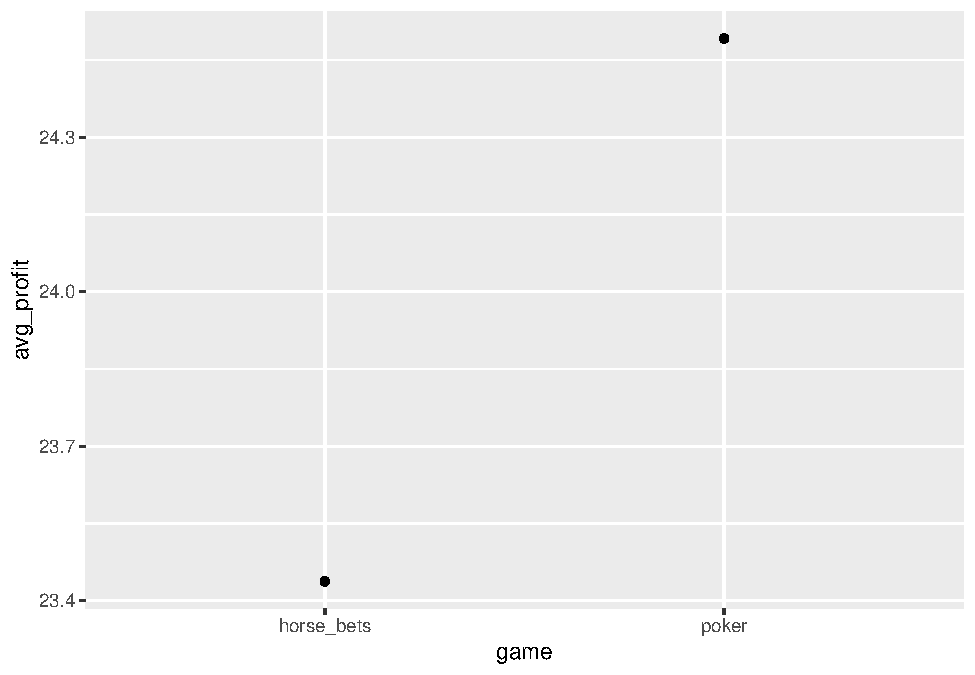
\includegraphics{main_files/figure-latex/unnamed-chunk-89-1.pdf}

\begin{itemize}
\tightlist
\item
  We may also want lines that connect the points.
\end{itemize}

\begin{Shaded}
\begin{Highlighting}[]
\FunctionTok{library}\NormalTok{(ggplot2)}
\FunctionTok{ggplot}\NormalTok{(profits\_by\_game\_and\_wday, }\FunctionTok{aes}\NormalTok{(game, avg\_profit, }\AttributeTok{color =}\NormalTok{ wday, }\AttributeTok{group =}\NormalTok{ wday)) }\SpecialCharTok{+} \FunctionTok{geom\_point}\NormalTok{() }\SpecialCharTok{+} \FunctionTok{geom\_line}\NormalTok{()}
\end{Highlighting}
\end{Shaded}

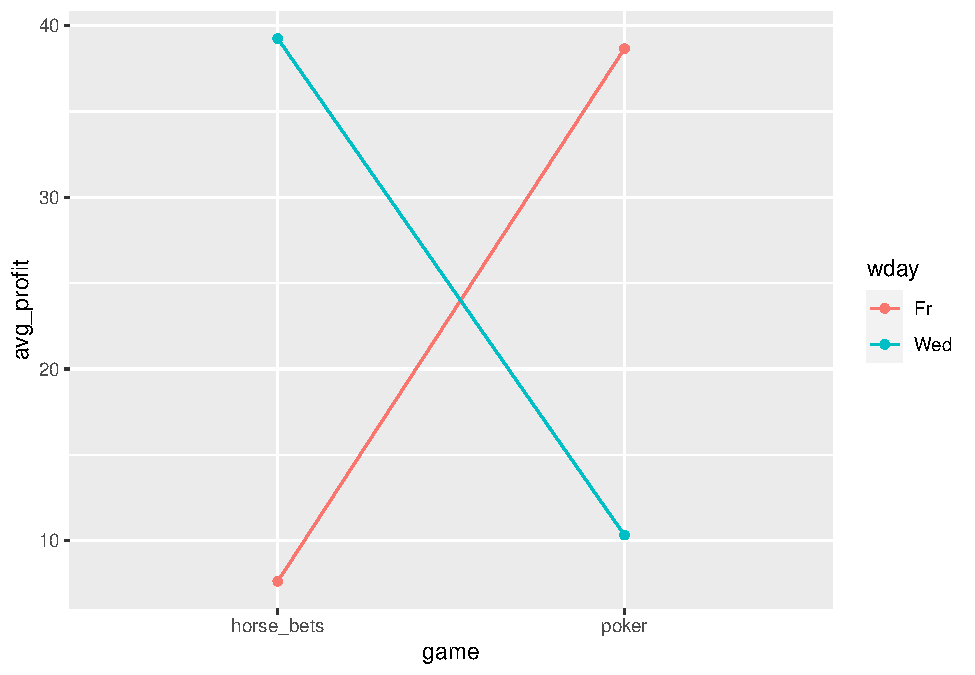
\includegraphics{main_files/figure-latex/unnamed-chunk-90-1.pdf}

\begin{itemize}
\tightlist
\item
  Or, we may want to have a bar graph.
\end{itemize}

\begin{Shaded}
\begin{Highlighting}[]
\FunctionTok{library}\NormalTok{(ggplot2)}
\FunctionTok{ggplot}\NormalTok{(profits\_by\_game, }\FunctionTok{aes}\NormalTok{(game, avg\_profit)) }\SpecialCharTok{+} \FunctionTok{geom\_bar}\NormalTok{(}\AttributeTok{stat =} \StringTok{"identity"}\NormalTok{)}
\end{Highlighting}
\end{Shaded}

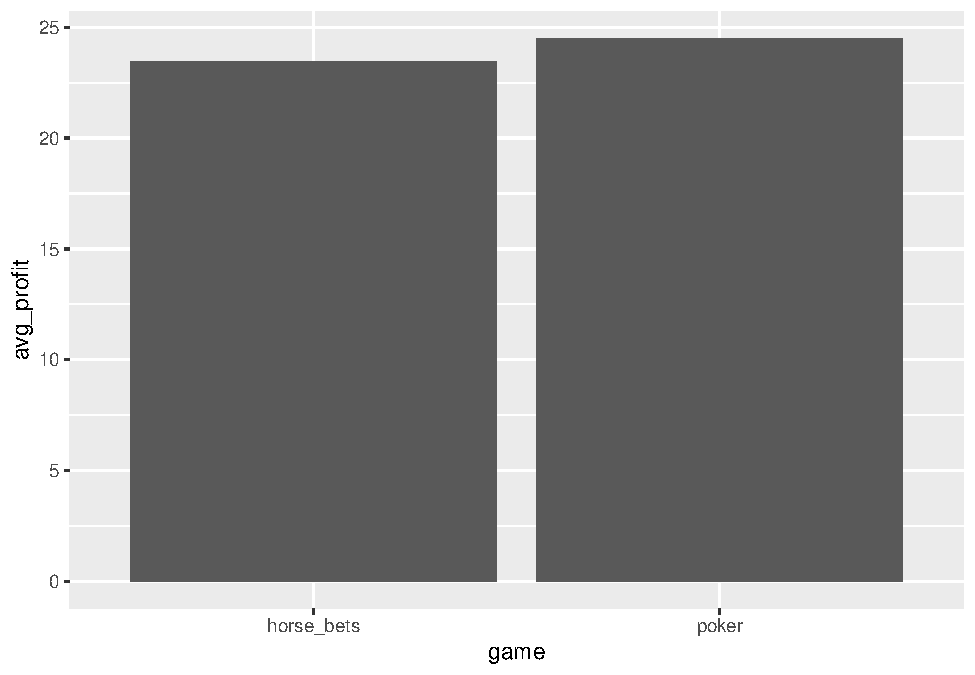
\includegraphics{main_files/figure-latex/unnamed-chunk-91-1.pdf}

\begin{Shaded}
\begin{Highlighting}[]
\FunctionTok{library}\NormalTok{(ggplot2)}
\FunctionTok{ggplot}\NormalTok{(profits\_by\_game\_and\_wday, }\FunctionTok{aes}\NormalTok{(game, avg\_profit, }\AttributeTok{fill =}\NormalTok{ wday)) }\SpecialCharTok{+} \FunctionTok{geom\_bar}\NormalTok{(}\AttributeTok{stat =} \StringTok{"identity"}\NormalTok{, }\AttributeTok{position =} \StringTok{"dodge"}\NormalTok{)}
\end{Highlighting}
\end{Shaded}

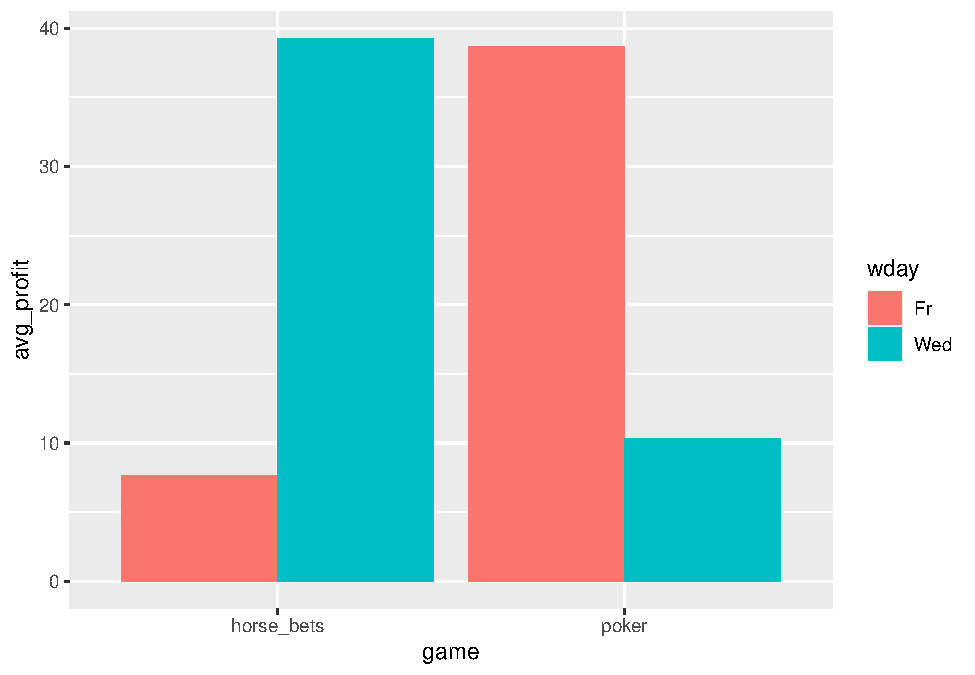
\includegraphics{main_files/figure-latex/unnamed-chunk-92-1.pdf}

\hypertarget{functions-in-this-section}{%
\section{Functions in this section}\label{functions-in-this-section}}

\texttt{data.frame(a\ =\ x,\ b\ =\ y,\ ...)}

Create a data frame from several vectors. The vectors can be different types.

\begin{itemize}
\tightlist
\item
  \texttt{x} A vector with \(n\) elements.
\item
  \texttt{y} Another vector with \(n\) elements.
\item
  \texttt{...} More vectors can be provided.
\end{itemize}

\texttt{View(x)}

Display a data frame, or another structure.

\texttt{head(df,\ n=6)}

Show the first \(n\) rows in the data frame df.

\begin{itemize}
\tightlist
\item
  \texttt{df} Data frame from which to display the first \(n\) rows.
\item
  \texttt{n} The number of rows to display. The default value for \(n\) is 6.
\end{itemize}

\texttt{sum(x)}

Compute the sum of a vector.

\texttt{length(x)}

Return the length of a vector.

\texttt{mean(x)}

Compute the mean of a vector.

\texttt{rep(x,\ n)}

Repeat the contents of a vector \(n\) times

\begin{itemize}
\tightlist
\item
  \texttt{x} The vector to be repeated.
\item
  \texttt{n} How many times to repeat the vector x.
\end{itemize}

\texttt{seq(from,\ to,\ by)}

Create a sequence of integers from \texttt{from} to \texttt{to} in steps of \texttt{by}.

\begin{itemize}
\tightlist
\item
  \texttt{from} The integer to start from.
\item
  \texttt{to} The integer to stop after.
\item
  \texttt{by} Size of steps to take. (If \texttt{from} \(>\) \texttt{to}, \texttt{by} needs to be negative.)
\end{itemize}

\texttt{rbind(df1,\ df2)}

Append df1 to df2 and return the resulting data frame. Both data frames need to have the same number of columns with the same names.

\begin{itemize}
\tightlist
\item
  \texttt{df1} First data frame.
\item
  \texttt{df2} Second data frame.
\end{itemize}

\hypertarget{working-with-data}{%
\chapter{Working with Data}\label{working-with-data}}

In this section, we learn how to work with data in a \textbf{dataframe}. A dataframe is a two-dimensional array consisting of \emph{rows} and \emph{columns}. You can simply think of it as a spreadsheet (e.g.~MS Excel, Google Sheets, etc.).

\hypertarget{basic-dataframes}{%
\section{Basic dataframes}\label{basic-dataframes}}

R has some prebuilt functions to build dataframes. Let us see a simple example. Consider the following three vectors.

\begin{Shaded}
\begin{Highlighting}[]
\NormalTok{name }\OtherTok{\textless{}{-}} \FunctionTok{c}\NormalTok{(}\StringTok{"Sam"}\NormalTok{, }\StringTok{"Paulina"}\NormalTok{, }\StringTok{"Cenk"}\NormalTok{)}
\NormalTok{age }\OtherTok{\textless{}{-}} \FunctionTok{c}\NormalTok{(}\DecValTok{23}\NormalTok{, }\DecValTok{34}\NormalTok{, }\DecValTok{19}\NormalTok{)}
\NormalTok{height }\OtherTok{\textless{}{-}} \FunctionTok{c}\NormalTok{(}\DecValTok{179}\NormalTok{, }\DecValTok{167}\NormalTok{, }\DecValTok{173}\NormalTok{)}
\end{Highlighting}
\end{Shaded}

Let us turn the data stored in different vectors into a single dataframe so that we can visualize the data better.

\begin{Shaded}
\begin{Highlighting}[]
\CommentTok{\#Let us first create the dataframe and assign it to the variable my\_df}
\NormalTok{my\_df }\OtherTok{\textless{}{-}} \FunctionTok{data.frame}\NormalTok{(name,age,height)}

\CommentTok{\#Let\textquotesingle{}s print the dataframe now}
\NormalTok{my\_df}
\end{Highlighting}
\end{Shaded}

\begin{Shaded}
\begin{Highlighting}[]
\NormalTok{\#\#      name age height}
\NormalTok{\#\# 1     Sam  23    179}
\NormalTok{\#\# 2 Paulina  34    167}
\NormalTok{\#\# 3    Cenk  19    173}
\end{Highlighting}
\end{Shaded}

We can select a particular row, column, or cell on a dataframe by using indices. For this we can use the slicing method \texttt{my\_dataframe{[}row,column{]}}.

\begin{Shaded}
\begin{Highlighting}[]
\CommentTok{\#Let us select the entire first row }
\NormalTok{my\_df[}\DecValTok{1}\NormalTok{,]}
\end{Highlighting}
\end{Shaded}

\begin{Shaded}
\begin{Highlighting}[]
\NormalTok{\#\#   name age height}
\NormalTok{\#\# 1  Sam  23    179}
\end{Highlighting}
\end{Shaded}

\begin{Shaded}
\begin{Highlighting}[]
\CommentTok{\#Now, let us select the first column }
\NormalTok{my\_df[,}\DecValTok{1}\NormalTok{]}
\end{Highlighting}
\end{Shaded}

\begin{Shaded}
\begin{Highlighting}[]
\NormalTok{\#\# [1] "Sam"     "Paulina" "Cenk"}
\end{Highlighting}
\end{Shaded}

\begin{Shaded}
\begin{Highlighting}[]
\CommentTok{\#Now, let us find Paulina\textquotesingle{}s height. For this, we need to get the 2nd row and 3rd column.}
\NormalTok{my\_df[}\DecValTok{2}\NormalTok{,}\DecValTok{3}\NormalTok{]}
\end{Highlighting}
\end{Shaded}

\begin{Shaded}
\begin{Highlighting}[]
\NormalTok{\#\# [1] 167}
\end{Highlighting}
\end{Shaded}

\begin{Shaded}
\begin{Highlighting}[]
\CommentTok{\#Now, let us find Paulina\textquotesingle{}s age and height. For this, we need to get the 2nd row and 2nd and 3rd columns.}
\NormalTok{my\_df[}\DecValTok{2}\NormalTok{,}\DecValTok{2}\SpecialCharTok{:}\DecValTok{3}\NormalTok{]}
\end{Highlighting}
\end{Shaded}

\begin{Shaded}
\begin{Highlighting}[]
\NormalTok{\#\#   age height}
\NormalTok{\#\# 2  34    167}
\end{Highlighting}
\end{Shaded}

\begin{Shaded}
\begin{Highlighting}[]
\CommentTok{\#Finally, let us get Sam and Paulina\textquotesingle{}s ages.}
\NormalTok{my\_df[}\DecValTok{1}\SpecialCharTok{:}\DecValTok{2}\NormalTok{,}\DecValTok{2}\NormalTok{]}
\end{Highlighting}
\end{Shaded}

\begin{Shaded}
\begin{Highlighting}[]
\NormalTok{\#\# [1] 23 34}
\end{Highlighting}
\end{Shaded}

You can also use the column name to select an entire column. Just add the dollar sign \texttt{\$} after the df and then the column mane.

\begin{Shaded}
\begin{Highlighting}[]
\NormalTok{my\_df}\SpecialCharTok{$}\NormalTok{age}
\end{Highlighting}
\end{Shaded}

\begin{Shaded}
\begin{Highlighting}[]
\NormalTok{\#\# [1] 23 34 19}
\end{Highlighting}
\end{Shaded}

\hypertarget{tibbles}{%
\section{Tibbles}\label{tibbles}}

The standard dataframes in R are good but not great. Often, we will deal with a lot of data we may not now which index to use to find the value we want. So, we need to be able to have some better ways to access data on our dataframes. We also want to be able to add new data or change some of the existing data easily. For this, we will use various packages in \textbf{tidyverse} for better dataframe management.

Let us first load the tidyverse library, which will load the necessary packages for the functionality described in the following sections.

\begin{Shaded}
\begin{Highlighting}[]
\FunctionTok{library}\NormalTok{(tidyverse)}
\end{Highlighting}
\end{Shaded}

Next, let us introduce tibbles. A \textbf{tibble} is a dataframe with some improved properties. We can turn a regular dataframe into a tibble by calling the \texttt{as\_tibble()} function on our dataframe.

\begin{Shaded}
\begin{Highlighting}[]
\CommentTok{\#Let\textquotesingle{}s turn my\_df into a tibble}
\NormalTok{my\_tibble }\OtherTok{\textless{}{-}} \FunctionTok{as\_tibble}\NormalTok{(my\_df)}

\CommentTok{\#Let\textquotesingle{}s print my\_tibble}
\NormalTok{my\_tibble}
\end{Highlighting}
\end{Shaded}

\begin{Shaded}
\begin{Highlighting}[]
\NormalTok{\#\# \# A tibble: 3 x 3}
\NormalTok{\#\#   name      age height}
\NormalTok{\#\#   \textless{}chr\textgreater{}   \textless{}dbl\textgreater{}  \textless{}dbl\textgreater{}}
\NormalTok{\#\# 1 Sam        23    179}
\NormalTok{\#\# 2 Paulina    34    167}
\NormalTok{\#\# 3 Cenk       19    173}
\end{Highlighting}
\end{Shaded}

As you can see above, the console output tells you that this is a 3x3 tibble meaning that it has 3 rows and 3 columns. It also tells you the type of the data in each column. You can see the data types right under each column name.

\hypertarget{beyond-toy-data}{%
\section{Beyond Toy Data}\label{beyond-toy-data}}

So far we have been working with toy data. In real life projects, you will have a lot more data. The data will usually be stored in some file from which you will have to read into a dataframe. Alternatively, it might be some dataset that from a corpus easily accessible to R. Let us see a few ways in which we can load some realistic datasets into a tibble.

\hypertarget{reading-data-from-a-csv-file}{%
\subsection{Reading data from a csv file}\label{reading-data-from-a-csv-file}}

In this course, we will use some of the data sets from Bodo Winter's book. Go to \href{https://osf.io/34mq9/}{this website} to download the \texttt{materials} folder. Once your data has been downloaded, navigate to the \texttt{materials/data} folder and locate the \texttt{nettle\_1999\_climate.csv} file.

To read in data from a csv to a tibble, we will use the \texttt{read\_csv()} function. All we need to do is to provide the path to the csv file we want to read in. If your csv file is in the same folder as your script, you can simply give its name. Otherwise, you need to provide the relevant directory information as well in your path.

\begin{Shaded}
\begin{Highlighting}[]
\CommentTok{\#Let\textquotesingle{}s read in the data}
\NormalTok{nettle }\OtherTok{\textless{}{-}} \FunctionTok{read\_csv}\NormalTok{(}\StringTok{\textquotesingle{}data/nettle\_1999\_climate.csv\textquotesingle{}}\NormalTok{)}
\end{Highlighting}
\end{Shaded}

\begin{verbatim}
## Rows: 74 Columns: 5
## -- Column specification --------------------------------------------------------
## Delimiter: ","
## chr (1): Country
## dbl (4): Population, Area, MGS, Langs
## 
## i Use `spec()` to retrieve the full column specification for this data.
## i Specify the column types or set `show_col_types = FALSE` to quiet this message.
\end{verbatim}

\begin{Shaded}
\begin{Highlighting}[]
\CommentTok{\#Let\textquotesingle{}s print the head of the data to see what it looks like}
\NormalTok{nettle}
\end{Highlighting}
\end{Shaded}

\begin{Shaded}
\begin{Highlighting}[]
\NormalTok{\#\# \# A tibble: 74 x 5}
\NormalTok{\#\#    Country      Population  Area   MGS Langs}
\NormalTok{\#\#    \textless{}chr\textgreater{}             \textless{}dbl\textgreater{} \textless{}dbl\textgreater{} \textless{}dbl\textgreater{} \textless{}dbl\textgreater{}}
\NormalTok{\#\#  1 Algeria            4.41  6.38  6.6     18}
\NormalTok{\#\#  2 Angola             4.01  6.1   6.22    42}
\NormalTok{\#\#  3 Australia          4.24  6.89  6      234}
\NormalTok{\#\#  4 Bangladesh         5.07  5.16  7.4     37}
\NormalTok{\#\#  5 Benin              3.69  5.05  7.14    52}
\NormalTok{\#\#  6 Bolivia            3.88  6.04  6.92    38}
\NormalTok{\#\#  7 Botswana           3.13  5.76  4.6     27}
\NormalTok{\#\#  8 Brazil             5.19  6.93  9.71   209}
\NormalTok{\#\#  9 Burkina Faso       3.97  5.44  5.17    75}
\NormalTok{\#\# 10 CAR                3.5   5.79  8.08    94}
\NormalTok{\#\# \# i 64 more rows}
\end{Highlighting}
\end{Shaded}

If you want to see the last 5 items, use the \texttt{tail()} function.

\begin{Shaded}
\begin{Highlighting}[]
\FunctionTok{tail}\NormalTok{(nettle)}
\end{Highlighting}
\end{Shaded}

\begin{Shaded}
\begin{Highlighting}[]
\NormalTok{\#\# \# A tibble: 6 x 5}
\NormalTok{\#\#   Country   Population  Area   MGS Langs}
\NormalTok{\#\#   \textless{}chr\textgreater{}          \textless{}dbl\textgreater{} \textless{}dbl\textgreater{} \textless{}dbl\textgreater{} \textless{}dbl\textgreater{}}
\NormalTok{\#\# 1 Venezuela       4.31  5.96  7.98    40}
\NormalTok{\#\# 2 Vietnam         4.83  5.52  8.8     88}
\NormalTok{\#\# 3 Yemen           4.09  5.72  0        6}
\NormalTok{\#\# 4 Zaire           4.56  6.37  9.44   219}
\NormalTok{\#\# 5 Zambia          3.94  5.88  5.43    38}
\NormalTok{\#\# 6 Zimbabwe        4     5.59  5.29    18}
\end{Highlighting}
\end{Shaded}

If you want to view the entire dataset, you can use \texttt{View(nettle)}. This will open a new tab in RStudio and show your data as a table.

\hypertarget{reading-data-from-r-data-packages}{%
\subsection{Reading data from R data packages}\label{reading-data-from-r-data-packages}}

R has various data packages you can install and use. Let us install the \texttt{languageR} which has some nice language datasets. Once you install the package and load the library, you can easily use the datasets as tibles. For all the details and available datasets in \texttt{languageR}, you can check the \href{https://cran.r-project.org/web/packages/languageR/languageR.pdf}{languageR documentation} on CRAN.

\begin{Shaded}
\begin{Highlighting}[]
\CommentTok{\#Let\textquotesingle{}s load the library}
\FunctionTok{library}\NormalTok{(languageR)}

\CommentTok{\#We\textquotesingle{}ll use the dativeSimplified dataset, which is documented. Let\textquotesingle{}s see the documentation}
\NormalTok{?dativeSimplified}
\end{Highlighting}
\end{Shaded}

\begin{Shaded}
\begin{Highlighting}[]
\CommentTok{\#let\textquotesingle{}s use the dativeSimplified data from the languageR }
\NormalTok{data }\OtherTok{\textless{}{-}} \FunctionTok{as\_tibble}\NormalTok{(dativeSimplified)}

\CommentTok{\#Let\textquotesingle{}s print the first few lines of the data}
\NormalTok{data}
\end{Highlighting}
\end{Shaded}

\begin{Shaded}
\begin{Highlighting}[]
\NormalTok{\#\# \# A tibble: 903 x 5}
\NormalTok{\#\#    RealizationOfRec Verb  AnimacyOfRec AnimacyOfTheme LengthOfTheme}
\NormalTok{\#\#    \textless{}fct\textgreater{}            \textless{}fct\textgreater{} \textless{}fct\textgreater{}        \textless{}fct\textgreater{}                  \textless{}dbl\textgreater{}}
\NormalTok{\#\#  1 NP               feed  animate      inanimate              2.64 }
\NormalTok{\#\#  2 NP               give  animate      inanimate              1.10 }
\NormalTok{\#\#  3 NP               give  animate      inanimate              2.56 }
\NormalTok{\#\#  4 NP               give  animate      inanimate              1.61 }
\NormalTok{\#\#  5 NP               offer animate      inanimate              1.10 }
\NormalTok{\#\#  6 NP               give  animate      inanimate              1.39 }
\NormalTok{\#\#  7 NP               pay   animate      inanimate              1.39 }
\NormalTok{\#\#  8 NP               bring animate      inanimate              0    }
\NormalTok{\#\#  9 NP               teach animate      inanimate              2.40 }
\NormalTok{\#\# 10 NP               give  animate      inanimate              0.693}
\NormalTok{\#\# \# i 893 more rows}
\end{Highlighting}
\end{Shaded}

\textbf{Dative Alternation} is the phenomenon in English where a recipient of a ditransitive verb can occur as an NP or a PP.

\begin{enumerate}
\def\labelenumi{\arabic{enumi}.}
\tightlist
\item
  Alex gave Sam a book.
\item
  Alex gave a book to Sam.
\end{enumerate}

Both of these constructions are grammatical and they mean essentially the same thing. The question is what factors are involved in picking one of the forms over the other. Bresnan et al.~(2007) used this data to determine the relevant factors.
Let us randomly select 10 examples and see what they look like. For that, we can use the folloing code.

\begin{Shaded}
\begin{Highlighting}[]
\CommentTok{\# store all possible row indices in a vector}
\NormalTok{indices\_all }\OtherTok{\textless{}{-}} \DecValTok{1}\SpecialCharTok{:}\FunctionTok{nrow}\NormalTok{(data)}

\CommentTok{\# set the random seed to make the results reproducible}
\FunctionTok{set.seed}\NormalTok{(}\DecValTok{123}\NormalTok{)}

\CommentTok{\# choose 10 such numbers at random without replacement}
\NormalTok{indices\_random }\OtherTok{\textless{}{-}} \FunctionTok{sample}\NormalTok{(indices\_all, }\AttributeTok{size =} \DecValTok{10}\NormalTok{)}

\CommentTok{\# use them to index the data frame to get the corresponding rows}
\NormalTok{data[indices\_random,]}
\end{Highlighting}
\end{Shaded}

\begin{Shaded}
\begin{Highlighting}[]
\NormalTok{\#\# \# A tibble: 10 x 5}
\NormalTok{\#\#    RealizationOfRec Verb  AnimacyOfRec AnimacyOfTheme LengthOfTheme}
\NormalTok{\#\#    \textless{}fct\textgreater{}            \textless{}fct\textgreater{} \textless{}fct\textgreater{}        \textless{}fct\textgreater{}                  \textless{}dbl\textgreater{}}
\NormalTok{\#\#  1 NP               give  inanimate    inanimate              1.79 }
\NormalTok{\#\#  2 NP               grant animate      inanimate              1.10 }
\NormalTok{\#\#  3 NP               grant animate      inanimate              2.40 }
\NormalTok{\#\#  4 NP               give  animate      inanimate              2.56 }
\NormalTok{\#\#  5 NP               tell  animate      inanimate              3.26 }
\NormalTok{\#\#  6 PP               give  animate      inanimate              0    }
\NormalTok{\#\#  7 NP               pay   animate      inanimate              0.693}
\NormalTok{\#\#  8 NP               hand  animate      inanimate              0.693}
\NormalTok{\#\#  9 NP               give  inanimate    inanimate              1.61 }
\NormalTok{\#\# 10 NP               wish  animate      inanimate              1.10}
\end{Highlighting}
\end{Shaded}

\hypertarget{summarizing-data}{%
\section{Summarizing Data}\label{summarizing-data}}

Looking at the summary statistics of your data is always a good first step. Let's take a look at the percentage of NP realizations of the recipient by animacy of the theme.

\begin{Shaded}
\begin{Highlighting}[]
\CommentTok{\# First, let\textquotesingle{}s take a look at the key dependet variable (NP or PP)}

\FunctionTok{unique}\NormalTok{(data}\SpecialCharTok{$}\NormalTok{RealizationOfRec)}
\end{Highlighting}
\end{Shaded}

\begin{Shaded}
\begin{Highlighting}[]
\NormalTok{\#\# [1] NP PP}
\NormalTok{\#\# Levels: NP PP}
\end{Highlighting}
\end{Shaded}

\begin{Shaded}
\begin{Highlighting}[]
\CommentTok{\# now, let\textquotesingle{}s compute the percentages (perc\_NP) and the number of observations in each subset}
\NormalTok{data}\SpecialCharTok{\%\textgreater{}\%} 
  \FunctionTok{group\_by}\NormalTok{(AnimacyOfRec) }\SpecialCharTok{\%\textgreater{}\%} 
  \FunctionTok{summarize}\NormalTok{(}\AttributeTok{perc\_NP =} \FunctionTok{mean}\NormalTok{(RealizationOfRec }\SpecialCharTok{==} \StringTok{"NP"}\NormalTok{), }
                   \AttributeTok{N =} \FunctionTok{n}\NormalTok{()}
\NormalTok{                  )}
\end{Highlighting}
\end{Shaded}

\begin{Shaded}
\begin{Highlighting}[]
\NormalTok{\#\# \# A tibble: 2 x 3}
\NormalTok{\#\#   AnimacyOfRec perc\_NP     N}
\NormalTok{\#\#   \textless{}fct\textgreater{}          \textless{}dbl\textgreater{} \textless{}int\textgreater{}}
\NormalTok{\#\# 1 animate        0.634   822}
\NormalTok{\#\# 2 inanimate      0.420    81}
\end{Highlighting}
\end{Shaded}

\textbf{What do the results say?}

\begin{itemize}
\tightlist
\item
  There are a total of 822 instances of animate recipients.
\item
  63\% of the animate recipients are NPs.
\end{itemize}

\hypertarget{working-with-dplyr}{%
\section{Working with dplyr}\label{working-with-dplyr}}

One of the packages in the \texttt{tidyverse} is \texttt{dplyr}. We use it to do various manipulations on the data frames. Check out the \href{https://nyu-cdsc.github.io/learningr/assets/data-transformation.pdf}{dplyr cheatsheet} for further details.

The \texttt{arrange} function will arrange your data in an ascending order.

\begin{Shaded}
\begin{Highlighting}[]
\FunctionTok{arrange}\NormalTok{(data)}
\end{Highlighting}
\end{Shaded}

\begin{Shaded}
\begin{Highlighting}[]
\NormalTok{\#\# \# A tibble: 903 x 5}
\NormalTok{\#\#    RealizationOfRec Verb  AnimacyOfRec AnimacyOfTheme LengthOfTheme}
\NormalTok{\#\#    \textless{}fct\textgreater{}            \textless{}fct\textgreater{} \textless{}fct\textgreater{}        \textless{}fct\textgreater{}                  \textless{}dbl\textgreater{}}
\NormalTok{\#\#  1 NP               feed  animate      inanimate              2.64 }
\NormalTok{\#\#  2 NP               give  animate      inanimate              1.10 }
\NormalTok{\#\#  3 NP               give  animate      inanimate              2.56 }
\NormalTok{\#\#  4 NP               give  animate      inanimate              1.61 }
\NormalTok{\#\#  5 NP               offer animate      inanimate              1.10 }
\NormalTok{\#\#  6 NP               give  animate      inanimate              1.39 }
\NormalTok{\#\#  7 NP               pay   animate      inanimate              1.39 }
\NormalTok{\#\#  8 NP               bring animate      inanimate              0    }
\NormalTok{\#\#  9 NP               teach animate      inanimate              2.40 }
\NormalTok{\#\# 10 NP               give  animate      inanimate              0.693}
\NormalTok{\#\# \# i 893 more rows}
\end{Highlighting}
\end{Shaded}

You can arrange the data based on a particular column. In that case, you need to provide the column name.

\begin{Shaded}
\begin{Highlighting}[]
\FunctionTok{arrange}\NormalTok{(data,LengthOfTheme)}
\end{Highlighting}
\end{Shaded}

\begin{Shaded}
\begin{Highlighting}[]
\NormalTok{\#\# \# A tibble: 903 x 5}
\NormalTok{\#\#    RealizationOfRec Verb   AnimacyOfRec AnimacyOfTheme LengthOfTheme}
\NormalTok{\#\#    \textless{}fct\textgreater{}            \textless{}fct\textgreater{}  \textless{}fct\textgreater{}        \textless{}fct\textgreater{}                  \textless{}dbl\textgreater{}}
\NormalTok{\#\#  1 NP               bring  animate      inanimate                  0}
\NormalTok{\#\#  2 NP               send   animate      inanimate                  0}
\NormalTok{\#\#  3 NP               bet    animate      inanimate                  0}
\NormalTok{\#\#  4 NP               tell   animate      inanimate                  0}
\NormalTok{\#\#  5 NP               tell   animate      inanimate                  0}
\NormalTok{\#\#  6 NP               give   inanimate    inanimate                  0}
\NormalTok{\#\#  7 NP               give   animate      inanimate                  0}
\NormalTok{\#\#  8 NP               charge animate      inanimate                  0}
\NormalTok{\#\#  9 NP               give   animate      inanimate                  0}
\NormalTok{\#\# 10 NP               pay    animate      inanimate                  0}
\NormalTok{\#\# \# i 893 more rows}
\end{Highlighting}
\end{Shaded}

\begin{Shaded}
\begin{Highlighting}[]
\FunctionTok{arrange}\NormalTok{(data[}\DecValTok{1}\SpecialCharTok{:}\DecValTok{10}\NormalTok{,], LengthOfTheme)}
\end{Highlighting}
\end{Shaded}

\begin{Shaded}
\begin{Highlighting}[]
\NormalTok{\#\# \# A tibble: 10 x 5}
\NormalTok{\#\#    RealizationOfRec Verb  AnimacyOfRec AnimacyOfTheme LengthOfTheme}
\NormalTok{\#\#    \textless{}fct\textgreater{}            \textless{}fct\textgreater{} \textless{}fct\textgreater{}        \textless{}fct\textgreater{}                  \textless{}dbl\textgreater{}}
\NormalTok{\#\#  1 NP               bring animate      inanimate              0    }
\NormalTok{\#\#  2 NP               give  animate      inanimate              0.693}
\NormalTok{\#\#  3 NP               give  animate      inanimate              1.10 }
\NormalTok{\#\#  4 NP               offer animate      inanimate              1.10 }
\NormalTok{\#\#  5 NP               give  animate      inanimate              1.39 }
\NormalTok{\#\#  6 NP               pay   animate      inanimate              1.39 }
\NormalTok{\#\#  7 NP               give  animate      inanimate              1.61 }
\NormalTok{\#\#  8 NP               teach animate      inanimate              2.40 }
\NormalTok{\#\#  9 NP               give  animate      inanimate              2.56 }
\NormalTok{\#\# 10 NP               feed  animate      inanimate              2.64}
\end{Highlighting}
\end{Shaded}

If you want to arrange things in a descending order, then you need to put the \texttt{desc()} function around the relevant column.

\begin{Shaded}
\begin{Highlighting}[]
\FunctionTok{arrange}\NormalTok{(data, }\FunctionTok{desc}\NormalTok{(LengthOfTheme))}
\end{Highlighting}
\end{Shaded}

\begin{Shaded}
\begin{Highlighting}[]
\NormalTok{\#\# \# A tibble: 903 x 5}
\NormalTok{\#\#    RealizationOfRec Verb  AnimacyOfRec AnimacyOfTheme LengthOfTheme}
\NormalTok{\#\#    \textless{}fct\textgreater{}            \textless{}fct\textgreater{} \textless{}fct\textgreater{}        \textless{}fct\textgreater{}                  \textless{}dbl\textgreater{}}
\NormalTok{\#\#  1 NP               give  inanimate    inanimate               3.64}
\NormalTok{\#\#  2 NP               send  animate      inanimate               3.56}
\NormalTok{\#\#  3 NP               give  animate      inanimate               3.53}
\NormalTok{\#\#  4 NP               pay   animate      inanimate               3.50}
\NormalTok{\#\#  5 NP               give  animate      inanimate               3.50}
\NormalTok{\#\#  6 NP               give  animate      inanimate               3.47}
\NormalTok{\#\#  7 NP               give  animate      inanimate               3.47}
\NormalTok{\#\#  8 NP               give  animate      inanimate               3.40}
\NormalTok{\#\#  9 NP               send  animate      inanimate               3.40}
\NormalTok{\#\# 10 NP               give  animate      inanimate               3.37}
\NormalTok{\#\# \# i 893 more rows}
\end{Highlighting}
\end{Shaded}

Another useful function is the \texttt{select()} function which allows you to create new dataframes using only columns you want.

\begin{Shaded}
\begin{Highlighting}[]
\CommentTok{\#Create the new dataframe using select}
\NormalTok{df }\OtherTok{\textless{}{-}} \FunctionTok{select}\NormalTok{(data, Verb, LengthOfTheme)}

\CommentTok{\#print the head}
\NormalTok{df}
\end{Highlighting}
\end{Shaded}

\begin{Shaded}
\begin{Highlighting}[]
\NormalTok{\#\# \# A tibble: 903 x 2}
\NormalTok{\#\#    Verb  LengthOfTheme}
\NormalTok{\#\#    \textless{}fct\textgreater{}         \textless{}dbl\textgreater{}}
\NormalTok{\#\#  1 feed          2.64 }
\NormalTok{\#\#  2 give          1.10 }
\NormalTok{\#\#  3 give          2.56 }
\NormalTok{\#\#  4 give          1.61 }
\NormalTok{\#\#  5 offer         1.10 }
\NormalTok{\#\#  6 give          1.39 }
\NormalTok{\#\#  7 pay           1.39 }
\NormalTok{\#\#  8 bring         0    }
\NormalTok{\#\#  9 teach         2.40 }
\NormalTok{\#\# 10 give          0.693}
\NormalTok{\#\# \# i 893 more rows}
\end{Highlighting}
\end{Shaded}

Another useful function is \texttt{sample\_n()} which randomly samples some number of datapoints.

\begin{Shaded}
\begin{Highlighting}[]
\FunctionTok{sample\_n}\NormalTok{(data, }\DecValTok{5}\NormalTok{)}
\end{Highlighting}
\end{Shaded}

\begin{Shaded}
\begin{Highlighting}[]
\NormalTok{\#\# \# A tibble: 5 x 5}
\NormalTok{\#\#   RealizationOfRec Verb  AnimacyOfRec AnimacyOfTheme LengthOfTheme}
\NormalTok{\#\#   \textless{}fct\textgreater{}            \textless{}fct\textgreater{} \textless{}fct\textgreater{}        \textless{}fct\textgreater{}                  \textless{}dbl\textgreater{}}
\NormalTok{\#\# 1 NP               give  animate      inanimate              0.693}
\NormalTok{\#\# 2 NP               sell  animate      inanimate              0    }
\NormalTok{\#\# 3 PP               give  animate      inanimate              1.61 }
\NormalTok{\#\# 4 PP               pay   animate      inanimate              1.39 }
\NormalTok{\#\# 5 PP               offer inanimate    inanimate              1.95}
\end{Highlighting}
\end{Shaded}

Two other useful functions are \texttt{group\_by()} and \texttt{ungroup()}.

\begin{Shaded}
\begin{Highlighting}[]
\CommentTok{\#Let\textquotesingle{}s group a small portion of the data by the realization of recipient}
\FunctionTok{group\_by}\NormalTok{(data[}\DecValTok{1}\SpecialCharTok{:}\DecValTok{5}\NormalTok{], RealizationOfRec)}
\end{Highlighting}
\end{Shaded}

\begin{Shaded}
\begin{Highlighting}[]
\NormalTok{\#\# \# A tibble: 903 x 5}
\NormalTok{\#\# \# Groups:   RealizationOfRec [2]}
\NormalTok{\#\#    RealizationOfRec Verb  AnimacyOfRec AnimacyOfTheme LengthOfTheme}
\NormalTok{\#\#    \textless{}fct\textgreater{}            \textless{}fct\textgreater{} \textless{}fct\textgreater{}        \textless{}fct\textgreater{}                  \textless{}dbl\textgreater{}}
\NormalTok{\#\#  1 NP               feed  animate      inanimate              2.64 }
\NormalTok{\#\#  2 NP               give  animate      inanimate              1.10 }
\NormalTok{\#\#  3 NP               give  animate      inanimate              2.56 }
\NormalTok{\#\#  4 NP               give  animate      inanimate              1.61 }
\NormalTok{\#\#  5 NP               offer animate      inanimate              1.10 }
\NormalTok{\#\#  6 NP               give  animate      inanimate              1.39 }
\NormalTok{\#\#  7 NP               pay   animate      inanimate              1.39 }
\NormalTok{\#\#  8 NP               bring animate      inanimate              0    }
\NormalTok{\#\#  9 NP               teach animate      inanimate              2.40 }
\NormalTok{\#\# 10 NP               give  animate      inanimate              0.693}
\NormalTok{\#\# \# i 893 more rows}
\end{Highlighting}
\end{Shaded}

Now let us group the data by verbs.

\begin{Shaded}
\begin{Highlighting}[]
\NormalTok{data\_grouped\_by\_verb }\OtherTok{\textless{}{-}} \FunctionTok{group\_by}\NormalTok{(data,Verb)}
\end{Highlighting}
\end{Shaded}

An important but complex function is the \texttt{summarize()} function.

\begin{enumerate}
\def\labelenumi{\arabic{enumi}.}
\tightlist
\item
  It divides a grouped data frame into subsets, with each subset corresponding to one value of the grouping variable (or a combination of values for several grouping variables).
\item
  It computes one or several values we specify on each such subset.
\item
  It creates a new data frame and puts everything together. The first column of this new data frame consists of levels of our grouping variable. In the following columns, the summarize() function prints the results of the computations we have specified.
\end{enumerate}

Try to guess the result of the following code. What will you see as an output? What will be the name of the columns?

\begin{Shaded}
\begin{Highlighting}[]
\CommentTok{\# summarize several variables}
\FunctionTok{summarize}\NormalTok{(data\_grouped\_by\_verb, }
          \AttributeTok{prop\_animate\_rec =} \FunctionTok{mean}\NormalTok{( AnimacyOfRec }\SpecialCharTok{==} \StringTok{"animate"}\NormalTok{ ),}
          \AttributeTok{prop\_animate\_theme =} \FunctionTok{mean}\NormalTok{( AnimacyOfTheme }\SpecialCharTok{==} \StringTok{"animate"}\NormalTok{ ),}
          \AttributeTok{N =} \FunctionTok{n}\NormalTok{()}
\NormalTok{          )}
\end{Highlighting}
\end{Shaded}

\begin{Shaded}
\begin{Highlighting}[]
\NormalTok{\#\# \# A tibble: 65 x 4}
\NormalTok{\#\#    Verb     prop\_animate\_rec prop\_animate\_theme     N}
\NormalTok{\#\#    \textless{}fct\textgreater{}               \textless{}dbl\textgreater{}              \textless{}dbl\textgreater{} \textless{}int\textgreater{}}
\NormalTok{\#\#  1 accord              1                      0     1}
\NormalTok{\#\#  2 allocate            0                      0     3}
\NormalTok{\#\#  3 allow               0.833                  0     6}
\NormalTok{\#\#  4 assess              1                      0     1}
\NormalTok{\#\#  5 assure              1                      0     2}
\NormalTok{\#\#  6 award               0.944                  0    18}
\NormalTok{\#\#  7 bequeath            1                      0     1}
\NormalTok{\#\#  8 bet                 1                      0     1}
\NormalTok{\#\#  9 bring               0.818                  0    11}
\NormalTok{\#\# 10 carry               1                      0     1}
\NormalTok{\#\# \# i 55 more rows}
\end{Highlighting}
\end{Shaded}

Try to interpret the output of the following code.

\begin{Shaded}
\begin{Highlighting}[]
\CommentTok{\# compute the averages}
\FunctionTok{summarize}\NormalTok{(data\_grouped\_by\_verb, }
          \AttributeTok{prop\_anim =} \FunctionTok{mean}\NormalTok{(AnimacyOfRec }\SpecialCharTok{==} \StringTok{"animate"}\NormalTok{),}
          \AttributeTok{prop\_inanim =} \DecValTok{1}\SpecialCharTok{{-}}\NormalTok{prop\_anim,}
          \AttributeTok{prop\_v\_recip\_anim =} \FunctionTok{ifelse}\NormalTok{(prop\_anim }\SpecialCharTok{\textgreater{}} \FloatTok{0.5}\NormalTok{, }\StringTok{"high"}\NormalTok{, }\StringTok{"low"}\NormalTok{)}
\NormalTok{          )}
\end{Highlighting}
\end{Shaded}

\begin{Shaded}
\begin{Highlighting}[]
\NormalTok{\#\# \# A tibble: 65 x 4}
\NormalTok{\#\#    Verb     prop\_anim prop\_inanim prop\_v\_recip\_anim}
\NormalTok{\#\#    \textless{}fct\textgreater{}        \textless{}dbl\textgreater{}       \textless{}dbl\textgreater{} \textless{}chr\textgreater{}            }
\NormalTok{\#\#  1 accord       1          0      high             }
\NormalTok{\#\#  2 allocate     0          1      low              }
\NormalTok{\#\#  3 allow        0.833      0.167  high             }
\NormalTok{\#\#  4 assess       1          0      high             }
\NormalTok{\#\#  5 assure       1          0      high             }
\NormalTok{\#\#  6 award        0.944      0.0556 high             }
\NormalTok{\#\#  7 bequeath     1          0      high             }
\NormalTok{\#\#  8 bet          1          0      high             }
\NormalTok{\#\#  9 bring        0.818      0.182  high             }
\NormalTok{\#\# 10 carry        1          0      high             }
\NormalTok{\#\# \# i 55 more rows}
\end{Highlighting}
\end{Shaded}

The last line uses the function ifelse(condition, value1, value2), which, for each element of the condition vector returns the corresponding element of the value1 vector if the condition is true at that element, or an element of vector2 otherwise.

mutate() proceeds similarly to summarize() in dividing a grouped dataset into subsets, but instead of computing one or several values for each subset, it creates or modifies a column.

The main difference between mutate() and summarize() is the output. While mutate() modifies the original and returns a modified version of it, summarize() creates a brand new data frame with one row for every combination of the the grouping variable values.

A very simple application of mutate() is to simply create a new column. In this case, we don't even need to group.

\begin{Shaded}
\begin{Highlighting}[]
\CommentTok{\# these two lines performs exactly the same action, }
\CommentTok{\# except the latter stores the result in df }
\NormalTok{data}\SpecialCharTok{$}\NormalTok{is\_realization\_NP }\OtherTok{\textless{}{-}}\NormalTok{ (data}\SpecialCharTok{$}\NormalTok{RealizationOfRec }\SpecialCharTok{==} \StringTok{"NP"}\NormalTok{ ) }
\NormalTok{df }\OtherTok{\textless{}{-}} \FunctionTok{mutate}\NormalTok{(data, }\AttributeTok{is\_realization\_NP =}\NormalTok{ (RealizationOfRec }\SpecialCharTok{==} \StringTok{"NP"}\NormalTok{) )}

\FunctionTok{head}\NormalTok{(df, }\DecValTok{2}\NormalTok{)}
\end{Highlighting}
\end{Shaded}

\begin{Shaded}
\begin{Highlighting}[]
\NormalTok{\#\# \# A tibble: 2 x 6}
\NormalTok{\#\#   RealizationOfRec Verb  AnimacyOfRec AnimacyOfTheme LengthOfTheme}
\NormalTok{\#\#   \textless{}fct\textgreater{}            \textless{}fct\textgreater{} \textless{}fct\textgreater{}        \textless{}fct\textgreater{}                  \textless{}dbl\textgreater{}}
\NormalTok{\#\# 1 NP               feed  animate      inanimate               2.64}
\NormalTok{\#\# 2 NP               give  animate      inanimate               1.10}
\NormalTok{\#\# \# i 1 more variable: is\_realization\_NP \textless{}lgl\textgreater{}}
\end{Highlighting}
\end{Shaded}

One final useful function is the \texttt{filter()} function. It allows you to find rows by particular values of a column.

\begin{Shaded}
\begin{Highlighting}[]
\FunctionTok{filter}\NormalTok{(data, is\_realization\_NP }\SpecialCharTok{==} \ConstantTok{FALSE}\NormalTok{)}
\end{Highlighting}
\end{Shaded}

\begin{Shaded}
\begin{Highlighting}[]
\NormalTok{\#\# \# A tibble: 348 x 6}
\NormalTok{\#\#    RealizationOfRec Verb  AnimacyOfRec AnimacyOfTheme LengthOfTheme}
\NormalTok{\#\#    \textless{}fct\textgreater{}            \textless{}fct\textgreater{} \textless{}fct\textgreater{}        \textless{}fct\textgreater{}                  \textless{}dbl\textgreater{}}
\NormalTok{\#\#  1 PP               give  animate      inanimate              0    }
\NormalTok{\#\#  2 PP               give  inanimate    inanimate              1.79 }
\NormalTok{\#\#  3 PP               give  animate      inanimate              1.39 }
\NormalTok{\#\#  4 PP               give  animate      inanimate              1.39 }
\NormalTok{\#\#  5 PP               sell  animate      inanimate              1.79 }
\NormalTok{\#\#  6 PP               give  inanimate    inanimate              0.693}
\NormalTok{\#\#  7 PP               give  inanimate    inanimate              0.693}
\NormalTok{\#\#  8 PP               give  animate      inanimate              1.39 }
\NormalTok{\#\#  9 PP               send  animate      inanimate              2.56 }
\NormalTok{\#\# 10 PP               offer animate      inanimate              1.95 }
\NormalTok{\#\# \# i 338 more rows}
\NormalTok{\#\# \# i 1 more variable: is\_realization\_NP \textless{}lgl\textgreater{}}
\end{Highlighting}
\end{Shaded}

\begin{Shaded}
\begin{Highlighting}[]
\FunctionTok{filter}\NormalTok{(data, LengthOfTheme }\SpecialCharTok{\textgreater{}} \FloatTok{3.5}\NormalTok{)}
\end{Highlighting}
\end{Shaded}

\begin{Shaded}
\begin{Highlighting}[]
\NormalTok{\#\# \# A tibble: 3 x 6}
\NormalTok{\#\#   RealizationOfRec Verb  AnimacyOfRec AnimacyOfTheme LengthOfTheme}
\NormalTok{\#\#   \textless{}fct\textgreater{}            \textless{}fct\textgreater{} \textless{}fct\textgreater{}        \textless{}fct\textgreater{}                  \textless{}dbl\textgreater{}}
\NormalTok{\#\# 1 NP               send  animate      inanimate               3.56}
\NormalTok{\#\# 2 NP               give  animate      inanimate               3.53}
\NormalTok{\#\# 3 NP               give  inanimate    inanimate               3.64}
\NormalTok{\#\# \# i 1 more variable: is\_realization\_NP \textless{}lgl\textgreater{}}
\end{Highlighting}
\end{Shaded}

\hypertarget{pipes}{%
\section{Pipes}\label{pipes}}

\hypertarget{the-problem}{%
\subsection{The problem}\label{the-problem}}

\begin{itemize}
\tightlist
\item
  The code below is really hard to read, even harder to maintain, and \texttt{dativeSimplified\_grouped\_by\_AnimacyOfRec\_and\_AnimacyOfTheme} is a terribly long variable name.
\end{itemize}

\begin{Shaded}
\begin{Highlighting}[]
\NormalTok{dativeSimplified\_grouped\_by\_AnimacyOfRec\_and\_AnimacyOfTheme }\OtherTok{\textless{}{-}}
      \FunctionTok{group\_by}\NormalTok{(dativeSimplified, AnimacyOfRec, AnimacyOfTheme)}
\NormalTok{df }\OtherTok{\textless{}{-}} \FunctionTok{summarize}\NormalTok{(dativeSimplified\_grouped\_by\_AnimacyOfRec\_and\_AnimacyOfTheme, }
                  \AttributeTok{perc\_NP =} \FunctionTok{mean}\NormalTok{(RealizationOfRec }\SpecialCharTok{==} \StringTok{"NP"}\NormalTok{) )}
\end{Highlighting}
\end{Shaded}

\begin{verbatim}
## `summarise()` has grouped output by 'AnimacyOfRec'. You can override using the
## `.groups` argument.
\end{verbatim}

\begin{Shaded}
\begin{Highlighting}[]
\NormalTok{df}
\end{Highlighting}
\end{Shaded}

\begin{Shaded}
\begin{Highlighting}[]
\NormalTok{\#\# \# A tibble: 4 x 3}
\NormalTok{\#\# \# Groups:   AnimacyOfRec [2]}
\NormalTok{\#\#   AnimacyOfRec AnimacyOfTheme perc\_NP}
\NormalTok{\#\#   \textless{}fct\textgreater{}        \textless{}fct\textgreater{}            \textless{}dbl\textgreater{}}
\NormalTok{\#\# 1 animate      animate          0.8  }
\NormalTok{\#\# 2 animate      inanimate        0.633}
\NormalTok{\#\# 3 inanimate    animate          1    }
\NormalTok{\#\# 4 inanimate    inanimate        0.412}
\end{Highlighting}
\end{Shaded}

\begin{itemize}
\tightlist
\item
  This alternative is also quite bad. To read this code, you need to know which bracket matches which other bracket.
\end{itemize}

\begin{Shaded}
\begin{Highlighting}[]
\NormalTok{df }\OtherTok{\textless{}{-}} \FunctionTok{summarize}\NormalTok{(}\FunctionTok{group\_by}\NormalTok{(dativeSimplified, AnimacyOfRec, AnimacyOfTheme), }
                  \AttributeTok{perc\_NP =} \FunctionTok{mean}\NormalTok{(RealizationOfRec }\SpecialCharTok{==} \StringTok{"NP"}\NormalTok{) )}
\end{Highlighting}
\end{Shaded}

\begin{verbatim}
## `summarise()` has grouped output by 'AnimacyOfRec'. You can override using the
## `.groups` argument.
\end{verbatim}

\begin{Shaded}
\begin{Highlighting}[]
\NormalTok{df}
\end{Highlighting}
\end{Shaded}

\begin{Shaded}
\begin{Highlighting}[]
\NormalTok{\#\# \# A tibble: 4 x 3}
\NormalTok{\#\# \# Groups:   AnimacyOfRec [2]}
\NormalTok{\#\#   AnimacyOfRec AnimacyOfTheme perc\_NP}
\NormalTok{\#\#   \textless{}fct\textgreater{}        \textless{}fct\textgreater{}            \textless{}dbl\textgreater{}}
\NormalTok{\#\# 1 animate      animate          0.8  }
\NormalTok{\#\# 2 animate      inanimate        0.633}
\NormalTok{\#\# 3 inanimate    animate          1    }
\NormalTok{\#\# 4 inanimate    inanimate        0.412}
\end{Highlighting}
\end{Shaded}

\begin{itemize}
\tightlist
\item
  One nested function call may be OK. But try to read this.
\end{itemize}

\begin{Shaded}
\begin{Highlighting}[]
\NormalTok{df }\OtherTok{\textless{}{-}}\NormalTok{ dplyr}\SpecialCharTok{::}\FunctionTok{summarize}\NormalTok{(}\FunctionTok{group\_by}\NormalTok{(}\FunctionTok{mutate}\NormalTok{(dativeSimplified, }\AttributeTok{long\_theme =} \FunctionTok{ifelse}\NormalTok{(LengthOfTheme }\SpecialCharTok{\textgreater{}} \FloatTok{1.6}\NormalTok{, }\StringTok{"long"}\NormalTok{, }\StringTok{"short"}\NormalTok{) ), long\_theme),}
              \AttributeTok{perc\_NP =} \FunctionTok{mean}\NormalTok{(RealizationOfRec }\SpecialCharTok{==} \StringTok{"NP"}\NormalTok{)}
\NormalTok{              )}
\end{Highlighting}
\end{Shaded}

\begin{itemize}
\tightlist
\item
  Or consider this expression (\texttt{sqrt} is the square root.)
\end{itemize}

\begin{Shaded}
\begin{Highlighting}[]
\FunctionTok{sqrt}\NormalTok{(}\FunctionTok{divide\_by}\NormalTok{(}\FunctionTok{sum}\NormalTok{(}\FunctionTok{divide\_by}\NormalTok{(}\DecValTok{2}\NormalTok{,}\DecValTok{3}\NormalTok{), }\FunctionTok{multiply\_by}\NormalTok{(}\DecValTok{2}\NormalTok{,}\DecValTok{3}\NormalTok{)), }\FunctionTok{sum}\NormalTok{(}\DecValTok{3}\NormalTok{,}\DecValTok{4}\NormalTok{)))}
\end{Highlighting}
\end{Shaded}

\begin{Shaded}
\begin{Highlighting}[]
\NormalTok{\#\# [1] 0.9759001}
\end{Highlighting}
\end{Shaded}

\begin{itemize}
\tightlist
\item
  Luckily, there a better way to write this expression.
\end{itemize}

\hypertarget{pipes-1}{%
\subsection{Pipes}\label{pipes-1}}

\begin{itemize}
\tightlist
\item
  The problem is that we have too many levels of embedding.
\item
  In natural language we avoid multiple embeddings of that sort by making shorter sentences, and using anaphors to refer to previous discourse.
\item
  The packages \textbf{dplyr} and \textbf{magrittr} provide a limited version of such functionality, and we'll need to use \textbf{pipe} operators (\texttt{\%\textgreater{}\%} and \texttt{\%\textless{}\textgreater{}\%}) to link expressions with an `anaphoric dependency'.
\item
  Whenever you see \texttt{\%\textgreater{}\%}, you can think about it as the following: ``Take whatever is on the left side, and use it in the function that is on the right side.''
\end{itemize}

\begin{Shaded}
\begin{Highlighting}[]
\FunctionTok{library}\NormalTok{(dplyr)}
\FunctionTok{library}\NormalTok{(magrittr)}
\CommentTok{\# Typical notation. Read as "Divide 10 by 2."}
\FunctionTok{divide\_by}\NormalTok{(}\DecValTok{10}\NormalTok{, }\DecValTok{2}\NormalTok{)}
\end{Highlighting}
\end{Shaded}

\begin{Shaded}
\begin{Highlighting}[]
\NormalTok{\#\# [1] 5}
\end{Highlighting}
\end{Shaded}

\begin{Shaded}
\begin{Highlighting}[]
\CommentTok{\# Equivalent pipe notation. Read as "Take 10, and divide it by 2."}
\DecValTok{10} \SpecialCharTok{\%\textgreater{}\%} \FunctionTok{divide\_by}\NormalTok{(., }\DecValTok{2}\NormalTok{)}
\end{Highlighting}
\end{Shaded}

\begin{Shaded}
\begin{Highlighting}[]
\NormalTok{\#\# [1] 5}
\end{Highlighting}
\end{Shaded}

\begin{Shaded}
\begin{Highlighting}[]
\CommentTok{\# Equivalent pipe notation. Read as "Take 2, and divide 10 by it."}
\DecValTok{2} \SpecialCharTok{\%\textgreater{}\%} \FunctionTok{divide\_by}\NormalTok{(}\DecValTok{10}\NormalTok{, .)}
\end{Highlighting}
\end{Shaded}

\begin{Shaded}
\begin{Highlighting}[]
\NormalTok{\#\# [1] 5}
\end{Highlighting}
\end{Shaded}

\begin{itemize}
\tightlist
\item
  If the dot operator occurs in the first argument slot, it can be omitted. (R has pro-drop.)
\end{itemize}

\begin{Shaded}
\begin{Highlighting}[]
\CommentTok{\# pipe notation with omission of \textquotesingle{}.\textquotesingle{}}
\DecValTok{10} \SpecialCharTok{\%\textgreater{}\%} \FunctionTok{divide\_by}\NormalTok{(}\DecValTok{2}\NormalTok{)}
\end{Highlighting}
\end{Shaded}

\begin{Shaded}
\begin{Highlighting}[]
\NormalTok{\#\# [1] 5}
\end{Highlighting}
\end{Shaded}

\begin{itemize}
\tightlist
\item
  Let's see how it can resolve the mess below. (Repetition of previous example.)
\end{itemize}

\begin{Shaded}
\begin{Highlighting}[]
\NormalTok{df }\OtherTok{\textless{}{-}} \FunctionTok{mutate}\NormalTok{(}\FunctionTok{group\_by}\NormalTok{(dativeSimplified, AnimacyOfRec, AnimacyOfTheme), }
                  \AttributeTok{perc\_NP =} \FunctionTok{mean}\NormalTok{(RealizationOfRec }\SpecialCharTok{==} \StringTok{"NP"}\NormalTok{) )}
\NormalTok{df}
\end{Highlighting}
\end{Shaded}

\begin{Shaded}
\begin{Highlighting}[]
\NormalTok{\#\# \# A tibble: 903 x 6}
\NormalTok{\#\# \# Groups:   AnimacyOfRec, AnimacyOfTheme [4]}
\NormalTok{\#\#    RealizationOfRec Verb  AnimacyOfRec AnimacyOfTheme LengthOfTheme perc\_NP}
\NormalTok{\#\#    \textless{}fct\textgreater{}            \textless{}fct\textgreater{} \textless{}fct\textgreater{}        \textless{}fct\textgreater{}                  \textless{}dbl\textgreater{}   \textless{}dbl\textgreater{}}
\NormalTok{\#\#  1 NP               feed  animate      inanimate              2.64    0.633}
\NormalTok{\#\#  2 NP               give  animate      inanimate              1.10    0.633}
\NormalTok{\#\#  3 NP               give  animate      inanimate              2.56    0.633}
\NormalTok{\#\#  4 NP               give  animate      inanimate              1.61    0.633}
\NormalTok{\#\#  5 NP               offer animate      inanimate              1.10    0.633}
\NormalTok{\#\#  6 NP               give  animate      inanimate              1.39    0.633}
\NormalTok{\#\#  7 NP               pay   animate      inanimate              1.39    0.633}
\NormalTok{\#\#  8 NP               bring animate      inanimate              0       0.633}
\NormalTok{\#\#  9 NP               teach animate      inanimate              2.40    0.633}
\NormalTok{\#\# 10 NP               give  animate      inanimate              0.693   0.633}
\NormalTok{\#\# \# i 893 more rows}
\end{Highlighting}
\end{Shaded}

\begin{itemize}
\tightlist
\item
  And here is the much more readable version of this code:
\end{itemize}

\begin{Shaded}
\begin{Highlighting}[]
\NormalTok{df }\OtherTok{\textless{}{-}}\NormalTok{  dativeSimplified }\SpecialCharTok{\%\textgreater{}\%}
          \FunctionTok{mutate}\NormalTok{(., }\AttributeTok{long\_theme =} \FunctionTok{ifelse}\NormalTok{(LengthOfTheme }\SpecialCharTok{\textgreater{}} \FloatTok{1.6}\NormalTok{, }\StringTok{"long"}\NormalTok{, }\StringTok{"short"}\NormalTok{) ) }\SpecialCharTok{\%\textgreater{}\%} 
          \FunctionTok{group\_by}\NormalTok{(., long\_theme) }\SpecialCharTok{\%\textgreater{}\%} 
\NormalTok{          dplyr}\SpecialCharTok{::}\FunctionTok{summarize}\NormalTok{(., }\AttributeTok{perc\_NP =} \FunctionTok{mean}\NormalTok{(RealizationOfRec }\SpecialCharTok{==} \StringTok{"NP"}\NormalTok{) )}
\end{Highlighting}
\end{Shaded}

\begin{itemize}
\tightlist
\item
  We don't actually need the dot:
\end{itemize}

\begin{Shaded}
\begin{Highlighting}[]
\NormalTok{df }\OtherTok{\textless{}{-}}\NormalTok{  dativeSimplified }\SpecialCharTok{\%\textgreater{}\%}
          \FunctionTok{mutate}\NormalTok{(}\AttributeTok{long\_theme =} \FunctionTok{ifelse}\NormalTok{(LengthOfTheme }\SpecialCharTok{\textgreater{}} \FloatTok{1.6}\NormalTok{, }\StringTok{"long"}\NormalTok{, }\StringTok{"short"}\NormalTok{) ) }\SpecialCharTok{\%\textgreater{}\%} 
          \FunctionTok{group\_by}\NormalTok{(long\_theme) }\SpecialCharTok{\%\textgreater{}\%} 
\NormalTok{          dplyr}\SpecialCharTok{::}\FunctionTok{summarize}\NormalTok{(}\AttributeTok{perc\_NP =} \FunctionTok{mean}\NormalTok{(RealizationOfRec }\SpecialCharTok{==} \StringTok{"NP"}\NormalTok{) )}
\end{Highlighting}
\end{Shaded}

\begin{itemize}
\tightlist
\item
  The \texttt{\%\textless{}\textgreater{}\%} operator is a convenient combination of \texttt{\%\textgreater{}\%} and \texttt{\textless{}-} which you can use to directly modify an object.
\end{itemize}

\begin{Shaded}
\begin{Highlighting}[]
\CommentTok{\# load the package magrittr in order to access the assignment pipe operator}
\FunctionTok{library}\NormalTok{(magrittr)}

\CommentTok{\# create a vector with numbers from 1 to 10}
\NormalTok{x }\OtherTok{\textless{}{-}} \DecValTok{1}\SpecialCharTok{:}\DecValTok{10}
\CommentTok{\# keep only numbers \textless{} 5:}
\CommentTok{\#   (i) without \%\textless{}\textgreater{}\%}
\NormalTok{x }\OtherTok{\textless{}{-}}\NormalTok{ x[x}\SpecialCharTok{\textless{}}\DecValTok{5}\NormalTok{]}
\CommentTok{\#   (i) with \%\textless{}\textgreater{}\%}
\NormalTok{x }\SpecialCharTok{\%\textless{}\textgreater{}\%}\NormalTok{ .[.}\SpecialCharTok{\textless{}}\DecValTok{5}\NormalTok{]}
\end{Highlighting}
\end{Shaded}

\begin{Shaded}
\begin{Highlighting}[]
\CommentTok{\# lets add several columns to \textquotesingle{}dativeSimplified\textquotesingle{}}
\NormalTok{dativeSimplified }\SpecialCharTok{\%\textless{}\textgreater{}\%} \FunctionTok{mutate}\NormalTok{(}\AttributeTok{A=}\DecValTok{1}\NormalTok{, }\AttributeTok{B=}\DecValTok{2}\NormalTok{, }\AttributeTok{C=}\DecValTok{3}\NormalTok{, }\AttributeTok{D=}\DecValTok{4}\NormalTok{)}
\FunctionTok{head}\NormalTok{(dativeSimplified)}
\end{Highlighting}
\end{Shaded}

\begin{Shaded}
\begin{Highlighting}[]
\NormalTok{\#\#   RealizationOfRec  Verb AnimacyOfRec AnimacyOfTheme LengthOfTheme A B C D}
\NormalTok{\#\# 1               NP  feed      animate      inanimate      2.639057 1 2 3 4}
\NormalTok{\#\# 2               NP  give      animate      inanimate      1.098612 1 2 3 4}
\NormalTok{\#\# 3               NP  give      animate      inanimate      2.564949 1 2 3 4}
\NormalTok{\#\# 4               NP  give      animate      inanimate      1.609438 1 2 3 4}
\NormalTok{\#\# 5               NP offer      animate      inanimate      1.098612 1 2 3 4}
\NormalTok{\#\# 6               NP  give      animate      inanimate      1.386294 1 2 3 4}
\end{Highlighting}
\end{Shaded}


  \bibliography{book.bib,packages.bib}

\end{document}
